\documentclass[12pt,twoside]{book}

%\usepackage{makeidx}
\RequirePackage{verbatim}
%\RequirePackage{alltt}
\usepackage{ifpdf}
\usepackage{etoolbox}
\usepackage{multicol}

\newtoggle{solutions}
\toggletrue{solutions}
\togglefalse{solutions}

\ifpdf
   \pdfcompresslevel=9
   \pdfoutput=1


   \usepackage[pdftex]{graphicx}
   \usepackage[pdftex]{geometry}
   \usepackage[pdftex]{color}
   \usepackage{hyperref}
   \hypersetup{
     pdftitle={Recitation Activities for the COMPASS program, Semester II},
     pdfsubject={ODE},
     pdfauthor={Kelly Black},
     pdfkeywords={classroom activities, calculus, physics},
     anchorcolor = {red},
     colorlinks = {true},
     %pdfpagemode={FullScreen}
   }
\else
   \usepackage{epsfig}
   \usepackage{color}
\fi

\usepackage{pgf}
\usepackage{pstricks}
\usepackage{tikz}
\usepackage{tikz-3dplot}
\usetikzlibrary{shapes,arrows.meta,bending}


\pagestyle{myheadings}

%\setlength{\basicoddside}{\oddsidemargin}
%\setlength{\basicevenside}{\evensidemargin}
%\setlength{\basicwidth}{\textwidth}
%\setlength{\basictop}{\topmargin}
%\setlength{\basicheight}{\textheight}


\input{header}
\setcounter{activity}{0}

\input{latexDefinitions}

\begin{document}


\title{Classroom Activities \\
  Semester II \\
  Coordinated Math-Physics Program
  \iftoggle{solutions}{%
    \\\textit{Solution Manual}
  }
}
\author{Kelly Black\\University of Georgia\\Department of Mathematics}

\maketitle

\noindent
Copyright (C)  2015-2017 Kelly Black

\noindent
Permission is granted to copy, distribute and/or modify this document
under the terms of the GNU Free Documentation License, Version 1.3
or any later version published by the Free Software Foundation;
with no Invariant Sections, no Front-Cover Texts, and no Back-Cover Texts.
A copy of the license is included in the section entitled "GNU
Free Documentation License".



\tableofcontents

%\clearpage


\chapter{Preliminaries}

\newcommand{\mlc}[1] {\texttt{>> #1 }}
\newcommand{\ttt}[1]{\texttt{#1}}

\section{MATLAB} 

\textbf{Note:} For a general introduction to MATLAB see \textit{The
  MATLAB User's Guide, Reference Manual}, or other \textit{MATLAB}
manuals.  You can buy the student edition of MATLAB.  It comes with a
good manual. \index{MATLAB}

If you are using MATLAB in other classes, you may consider buying the 
\textbf{MATLAB Guide} by Desmond J. Higham and Nicholas J. Higham, published
by Siam.  

\subsection{Basic operations} Examples of common tasks are given
below.  Try interactively typing these commands at the command prompt
to get a sense of the environment as well as the language. The
command 'Press Enter' is abbreviated by ENTER.

\vspace{2em}


\begin{tabular}{lll} 
  \ttt{>>} 3+5     &ENTER   &Add two numbers and display results. \\ 
  \ttt{>>} 4-6     &ENTER   &Subtract two numbers and display results. \\ 
  \ttt{>>} 4-6;    &ENTER   &Subtract two numbers and do NOT
  display results.\\
  \ttt{>>} a = 12/5; &ENTER   &Divide and store result in variable 'a'.\\
  \ttt{>>} a        &ENTER  &Display content of variable 'a'. \\
  \ttt{>>} 1:2:11   &ENTER  &Generate a list of values. \\
  \ttt{>>} b=1:0.1:2 &ENTER & Fill an array with values from 1 to
  2 in increments of 0.1.\\
  \ttt{>>} b          &ENTER & Display content of 'b'. \\
  \ttt{>>} who      &ENTER  &List current variables. \\
  \ttt{>>} whos     &ENTER  &List current variables and their size.\\
  \ttt{>>} d = 5:1:15 &ENTER &Fill array 'd'. \\
  \ttt{>>} b + d     &ENTER &Add two arrays. \\
  \ttt{>>} b .* d    &ENTER & Multiply two arrays component wise. \\
  \ttt{>>} b * d     &ENTER & \\ 
  \ttt{>>} g = [1 2; 3 4; 5 6] &ENTER &Define a two dimensional array. \\
  \ttt{>>} g2 = 2*g  &ENTER & Multiply array by a constant. \\
\end{tabular}

\subsection{Plotting Examples}  ~

\begin{tabular}{lll}
  \ttt{>>} \verb!x = -5:0.1:5;!  &ENTER  &Set up the independent variable. \\
  \ttt{>>} y = \verb!x.^2!; &ENTER  & Compute dependent variable or
  y-values . \\ 
  \ttt{>>} z = \verb!(1/8)*x.^3!;      &ENTER  & Compute values for
  a second function. \\ 
  \ttt{>>} plot(x,y);     &ENTER  & Plot x versus y. \\
  \ttt{>>} hold on;      &ENTER &Hold current graph . \\
  \ttt{>>} plot(x,z,'r'); &ENTER &Plot graph of 'z', in red, on same
  axis as 'y', \\
  \ttt{>>} title('y, z, versus x'); & ENTER & Set the title for the
  plot. \\
  \ttt{>>} hold;         &ENTER &Release current plot.  Next plot
  property is 'replace'. \\ 
\end{tabular}

\subsection{Sums, Loops, and Variables} ~ 

\begin{tabular}{lll}
  \ttt{>>} u = [ 1 2 3 4 5]  &ENTER &Define the row vector 'u'. \\
  \ttt{>>} v = [ 6 7 8 9 10 ]' &ENTER &Define the column vector 'v'.\\
  \ttt{>>} w = (1:0.2:20)' &ENTER & Define the column vector 'w'. \\
  \ttt{>>} whos     &ENTER &Check the dimensions of the vectors. \\
  \ttt{>>} help sum &ENTER &  Example:  Get help with the
  SUM command. \\ 
  \ttt{>>} sum(v,1) &ENTER &Add values of  vector 'v'.\\
  \ttt{>>} sum(u,1) &ENTER &Observe results. \\ 
  \ttt{>>} sum(u,2) &ENTER & Add values of vector 'v'. \\
  \ttt{>>} \%  This is a comment line  &ENTER & \\  
  \ttt{>>} \%  Next we will try a for loop. &ENTER & \\
  \ttt{>>} clear x; &ENTER &  clear x-variable.  \\      
  \ttt{>>} n = 10;  &ENTER &Set up loop limit. \\
  \ttt{>>} for i = 1:n, x(i) = i+1, end  &ENTER  & \\
  \ttt{>>} x   &ENTER &Display content of vector 'x'. \\
  \ttt{>>} clear &ENTER & Clear all variables. \\
\end{tabular}

\subsection{Editing and running M-files} You can do many useful computations
working entirely at the MATLAB command line, but soon you will find it helpful
to save a list of commands to an M-file.  M-file are the equivalents of programs
functions, subroutines, and procedures in other programming languages.

An M-file is a text file that has a \textbf{.m} filename extension and contains 
MATLAB commands.

There are two types:
\begin{itemize}
  \item{\textbf{Script M-files}} (or command files) have no input or output
  arguments and operate on variables in the workspace.  A script enables you to
  store a sequence of commands that are to be used repeatedly or will be needed
  at some future time.
  
  \item{\textbf{Function M-files}} contain a function definition line and can
  accept input arguments and return output arguments and their internal
  variables are local to the function (unless declared global).
\end{itemize}

\begin{enumerate}
  \item To create an M-file click on the "new file" icon \textbf{or}\\
  $\rightarrow$ Select File
  
  \hspace{.2in}$\rightarrow$  Select New 
  
  \hspace{.4in}$\rightarrow$  Select M-file\\
  A text edit window will open.
  
  \item Enter the following MATLAB commands to create a MATLAB script.\\
  \verb!% Plot the function y=x^2.!\\
  \verb!% This is my first M-file experience!\\
  \ttt{x=-5:0.001:5;}\\
  \verb!y=x.^2;!\\
  \ttt{plot (x,y)}
  
  \item Save the M-file to a convenient folder as test1.m.
  
  If this is the first time you are running MATLAB, you may need to create the
  folder "Calculus."
  
  When MATLAB opens, a default directory is used.  To change the
  directory click on the icon to the right of the displayed directory
  name.  The "Browse for Folder"
  window will open.\\
  $\rightarrow$ Click on the drive you want to use.\\
  $\rightarrow$ Click on the sequence of folder icons to get to the
  folder that you wish to use.\\
  $\rightarrow$ Now save your M-file to the folder "Calculus."
  
  \item To execute the MATLAB script click on the "Save and Run" or "Run" icon. 
  The first time you select the "Run" command the MATLAB Editor window
  you may be asked to switch to the current directory. If so then
  choose the option to use the directory.
  
  If you get a message that the file was not found then you can select
  on of the following:
  \begin{itemize}
    \item Change MATLAB current directory
    \item Add directory to the top of the MATLAB path
    \item Add directory to the bottom of the MATLAB path.
  \end{itemize}
  Select "Add directory to the top of the MATLAB path" and click on
  OK.  MATLAB will then execute the script.

  What do you observe?
  
  \item Next create a function called f1.m that will generate the points to plot
  the function $f(x)=e^{(-x/3)}\sin(2x)$ using M-file.
  
  Open a new M-file and type the following commands:
  \begin{verbatim}
    function y=f1(x)
    % y=f1(x) : This is my second M-file experience
    y=exp(-x/3).*sin(2*x);
  \end{verbatim}
  Save the file as f1.m to the same folder used above.
  
  To execute the function we first need to define $x$.  Return to the command
  window and define $x$  and execute the function as follow:\\
  \begin{verbatim}
    >> x1=-5:0.01:5;
    >> y1=f1(x1); % execute function
    >> plot(x1,y1)
  \end{verbatim}
  
  MATLAB has a help command that can be invoked.  The MATLAB help function outputs
  all the comment lines before the first blank line in an M-file.  Enter\\
  \mlc{help f1}\\
  The last example was a function with a single input and one output.  A function
  can include more than one input or output.  The next example will construct a
  function with one input and two outputs.
  
  Open a new M-file and type the following commands:
  \begin{verbatim}
    function [y,z]=f2(x)
    %[y,z]=f2(x)  My third M-file.
    y=exp(-x/3).*sin(2*x);
    z=exp(-x/3).*cos(2*x);
  \end{verbatim}
  Save the file as f2.m to the same folder used above.
  
  To execute this function and to plot the output type the following commands in 
  the command window:\\
  \mlc{[y1,z1]=f2(x1);}\\
  \mlc{plot(x1,[y1,z1])}\\
  
  \item Our next example is a more complex M-file script.  Functions are like
  subroutines in that they have their own internal variables and communicate
  with the command window and the workspace through their inputs and outputs. 
  Scripts, on the other hand, are simply sequences of commands which operate on
  the variables in the workspace.  Any variable created in a script is placed in
  the workspace.  For that reason it is good practice to clear any variables
  which are no longer needed.  Scripts do not use inputs or create outputs and
  will give an error if you ask for it.  (Functions need not have outputs
  however.)  We will call the script f2\_plot.m.
  
  Open a new M-file and type the following commands:
  \begin{verbatim}
    % f2_plot	(Note: Not a "function" so first line can be a comment)
    % Script to plot output of function f2    
    [u,v] = f2(x1);
    figure(1)
    subplot(2,1,1); plot(x1,[u,v]);
    title('u, v versus x');
    xlabel('x1');
    ylabel('Feet');
    w = u.*v;
    z = u.^2+v.^2;
    subplot(2,1,2); plot(x1,[w,z]);
    title('w, z versus x');
    xlabel('x1');
    ylabel('Sq. Feet');
    clear u v w z
  \end{verbatim}
  Save the M-file as f2\_plot.m to the same folder used above.
  
  To execute the M-file script either click on the "Run" icon or type f2\_plot
  at the \ttt{>>} command prompt in the command window.
  
  What do you observe?  What effect does the subplot command have?
  \vspace{.25in}
  
  \item We will do one more example of a function.  This function will create a
  sequence of numbers, called the Fibonacci sequence.  It will have one input
  and one output and use a "for" loop to generate the sequence.

  Open a new M-file type the following commands including the comments:
  \begin{verbatim}
    function y=fibonacci(n)
    % y=fibonacci(n)
    % Populate the vector y with the first n terms of the Fibonacci sequence,
    % using a "for" loop.
    % The sequence is named after the Italian mathematician Leonardo Pisano,
    % nicknamed Leonardo Fibonacci, who lived about 1175-1250 AD.
    % After the second term, the Fibonacci sequence is generated by adding the
    two previous terms to generate the current term.
    y(1)=1;
    y(2)=1;
    for i=3:n
        y(i)=y(i-1)+y(i-2);
    end
  \end{verbatim}
  Save the M-file as fibonacci.m in the same folder used previously.
  
  To display the comments at the beginning of the fibonacci.m file and to
  execute it, type the following commands in the command window:
  \begin{verbatim}
  >>help fibonacci
  >>n=5
  >>y1=fibonacci(n)
  \end{verbatim}
  
  If you would like to plot the sequence type the following commands in the
  command window:
  \begin{verbatim}
  >>n=1:1:12;
  >>n1=12;
  >>y=fibonacci(n1);
  >>plot(n,y,'*')
  \end{verbatim}
  What do you observe?
  
     
\end{enumerate}



\section{Assignment Guidelines}


\subsection{Home Work} \index{Home Work}
All work that is handed in for a grade must be neat. Any work that
cannot be easily read will not be graded. Every home work assignment
must have your name at the top of every page and all sheets must be
stapled together. Assignments that are not stapled will have points
deducted.

The front page must have your name written on it. The front page must
also have three other items. First, the current assignment should be
written. Secondly, it should have the times that you planned in
advance to work on the homework. Third, it should have the times that
you did the actual work.

Each page must be one column. Your solutions to the home work problems
should be written out one after the other and not on the same line.
For example, after completing a problem the next problem should appear
directly below the previous problem. Once you reach the bottom of the
page you must move on to the next page and not start over in a second
column on the current page.

A front page should look like the following: \\
\begin{center}
\fbox{
\begin{minipage}[h]{4in}
Stuart Dent \\
Page 32 1-5 odd, 27, 29, and 35. \\
Page 107 21-31 odd, 35a, and 42. 

\vspace{2em}

Original times: Tuesday 5-6pm, Wednesday 4:30-5:30, and Thursday
6-7pm.

\vspace{2em}

Actual times: Thursday 8pm to Friday 2am.

\vspace{2em}

Page 32: \\
1) $\frac{d}{dt} t^2 = 2t$.

3) $\frac{d}{dt} \left( \sqrt{t} + t \right)  = 
    \frac{1}{2} t^{-\frac{1}{2}} + 1$

$\vdots$

\end{minipage}}
\end{center}

\subsection{Group Work} \index{Group Work}
For many of the assignments in this class you will be required to work
in small groups.  Please keep in mind the following guidelines when
taking part in group work: \index{group work}
\begin{enumerate}
\item Cooperate with each other. Work together and find a solution to
  the problem together.

\item Make sure that everyone understands each answer before the group
  moves on to the next question.

\item Listen carefully to each other and try, whenever possible, to
  build upon their ideas.

\item Share in the leadership of the group.  You may wish to assign
  different roles, i.e. moderator, recorder, etc., to different
  individuals.
  
\item Make sure that everyone participates and that no one dominates.
  If you see someone in the group who is lost, urge him or her to ask
  questions, or ask a simple question yourself to bring others into
  the discussion.

\item Ask questions when you don't understand something.

\item Do not be critical of other people's \textbf{questions}.
\end{enumerate}



\subsection{Projects} \index{Projects}
Formal projects will be assigned in this class. You will have between
one and two weeks to complete each project. You will either present
the project in a presentation in front of the class or turn in a
written report. 

Before the due date of the project you must meet with your professor
at least twice. All members of your group should be present at the
meeting. Meetings should be scheduled at the beginning of project work
on the Friday that projects are handed out.  \index{meeting} Your
group needs to meet for at least an hour before this meeting. The
total length of the meeting is 30 minutes. After 30 minutes the
meeting is concluded.

\subsubsection {Rewrites}
Written submissions can be rewritten and resubmitted within a week
after they are turned back to you.  \index{written projects} You may be
able to increase your grade significantly with a modicum of extra work
by using our suggestions to improve the quality of the presentation.


\subsubsection{Outline for the Written  or Oral Presentation}

The formal write up for this lab should be about five pages long and
should be typed. \index{written projects} But we will be more
concerned about whether or not the key questions are answered rather
than the length of the write up.  The text should be double spaced. Be
sure that {\it every} member of the group signs the lab report.  By
signing your name, you are indicating that you contributed
significantly toward the completion of that report.


Your report should include the topics given in the outline below.  You
do not have to follow the outline, but your report should address all
of the issues listed in the outline.  (For some reports the sample
outline may not be appropriate!)

%\begin{table}[hb]
\begin{itemize}
\index{written projects}
\item Title Page -- should include the following (in order):
  \begin{itemize}
  \item Title
  \item Date
  \item The typed name and signature of each member (on separate
    lines).
  \end{itemize}
\item Abstract -- A brief summary of the project
\item Introduction
  \begin{itemize}
  \item Very briefly describe the situation, finer details are given
     later.  Restate the problem in a way that points to a solution method.
     %(For example, Can we find reasonable and believable accelerations
     %and wait times for Joe and his mom that give Joe's travel time to
     %be 5 seconds less than his mom without Joe speeding.)
   \item Explicitly state your findings.  (You are expected to justify
     these findings in the sections that follow.)
  \end{itemize}

\item Physical Situation
  \begin{itemize}
  \item Include a full description of the physical system.
  \item Carefully define all of the important qualitative aspects.
  \item Include appropriate visualizations of the problem (e.g. graphs,
        free body diagrams).
  \item Be very careful about the flow of this part of your report. If
        the transitions are awkward we will take off points!
  \end{itemize}

\item Mathematical Model
  \begin{itemize}
  \item Describe and state the problem in mathematical terms.  Justify
    your plan of attack.
  \item  Discuss and justify any assumptions made.
  \item Include any other important definitions.
  \item  Present the details of your calculations.  Discuss clearly what you
    are doing at each step and why.
  \item Support your conclusions! A statement which is not carefully
    and correctly explained will not receive credit.
  \item Provide appropriate and convincing checks.
  \end{itemize}

\item Conclusion
  \begin{itemize}
  \item Include a brief description of the physical system.
  \item Briefly describe methods used to obtain result.
  \item Restate your findings and give a brief description of what is
    happening.
  \end{itemize}


\end{itemize}

%\caption{Sample Outline.}
%\label{sampleOutline}
%\end{table}


\subsubsection{Grade}

Your grade will be determined by the content and mechanics of your
final report. \index{grading} The only way that we have to determine
whether or not you understand the concepts discussed in class is
through the way in which you communicate your understanding of the
concepts. The primary goal of this exercise is for you to demonstrate,
through the process of a formal write-up, that you can effectively
communicate complex ideas. We will pay close attention to the
following aspects of your write-up:
\begin{itemize}
\index{grading}
\item Content \& Accuracy (75\%) \\
    This score is based on your answers to the questions and general
    technical merit of the report.
    \begin{enumerate}
    \item The paper should be written so that someone who is
      currently taking calculus should be able to read the paper,
      understand the problem, and understand the solution
      without having seen this handout.
      {\em The paper should stand by itself}.
    \item All of the important concepts should be included and
      defined.
    \item All statements should be supported. A statement without
      justification is not acceptable.
    \item The paper should not be a disjoint collection of
      statements. We expect you to demonstrate that you know how the
      different concepts relate to one another and clearly present
      how one idea is related to and leads to another idea.
    \item All of the items listed above in the report outline should
      be included.
    \end{enumerate}

  \item Mechanics \& Presentation (25\%)  \\
    This score will be based on overall organization, neatness,
    grammar, and spelling.
    \begin{enumerate}
    \item We will count off if the grammar or spelling is so poor that
      we cannot easily understand the paper.
    \item The overall flow of the paper is important.
    \item Pay careful attention to transitions.  Transitions are
      statements that let the reader know why you are discussing what
      you are discussing.
    \end{enumerate}


\end{itemize}


\section{Oral Presentations}

\subsection{Introduction}
To help you prepare for your talk we would like to share a few helpful
tips. \index{presentations} The tips range from how to structure your
talk to some specific pointers. Please look over this document before
giving your talk and consider the hints while you are working on your
project.

\section{Mechanics}
First, we will provide a few pointers on some of the mechanics of a
talk. The mechanics are very important and are something that you will
have to practice.

\subsubsection{Starting Your Talk} Do not assume that everybody in the
room knows what your talk is going to be about! Give a brief overview
of what is happening. The overview should only take three to four
sentences and absolutely no more. \index{presentations!introduction}

Once you have let your audience know \textit{what} you will talk
about, let them know \textit{how} you will approach the problem.
Provide an outline for the talk. Explicitly state the different steps
in the problem and state who will be discussing which part of your
talk. The outline will help your audience as you make the transitions
throughout the presentation.

\subsubsection{Physical Situation}
Do not assume that everybody in the room knows what is going on!
\index{presentations|introduction} After providing an outline, provide
a description of the physical problem and state all of your
assumptions. Several of the people in the room have not seen the
problem in over a week and probably did not think real hard about it
in the first place.

\subsubsection{Who Are You Talking To?}  Face the audience when you are
talking and do not block the board. It is easy to get wrapped up with
the equations on the board, but do not forget that you are trying to
share your information with the rest of the class. Face the class and
speak in a loud clear voice. The people in the back of the room would
like to hear you.

(Tip: when I am in front of a class I find it hard to keep
the equations straight, avoid blocking what I am writing, make eye
contact with people, and project my voice all at the same time.
Sometimes, with complicated derivations, I just look at the back of
the room and try to project my voice on the back wall.)

\subsubsection{Transitions} Moving from one topic to another in the
middle of a presentation can be difficult for you, but do not forget
that it is even more difficult for your audience. Be aware of the
places in which you move from one topic to another. When this occurs,
give a brief, one or two sentence review of what you just covered and
explicitly tell them that you will be moving to the next topic.
\index{presentations!transitions}

You should provide an outline at the beginning of the talk, and you
should provide an outline for each little section in your talk as
well. As you move through the different topics in your talk, it is a
good thing to remind people of the big picture, and you should also
remind them of what you will be doing.

\subsubsection{Practice, Practice, Practice}
Practice your presentation. Practice by yourself and pay careful
attention to the timing. You should also practice with the rest of the
group. It is quite difficult to get a smooth transition when you are
passing off the speaking position to another person. Practice this!

\textit{When you practice, always keep a clock in clear view.}


\section{Mathematics}
Presenting mathematics to a group of people is a perilous game.
\index{presentations!mathematics} Some people do not want to know
details, some people do, some people just do not care, some people
care passionately, and some people are afraid. You will always have to
make decisions on how to balance your talk.

\subsubsection{Difficult Formulas} The world is a terribly complicated
place. Unfortunately, it is very rare to come across physical phenomena
that follow simple mathematical functions. To make matters worse, the
operations that are performed (derivatives, integrals, differential
equations, etc.) pervert the formulas into even more difficult forms.
When this happens, you cannot put every detail on the board and expect
your audience to follow what you are doing.

So what do you do when you have long, difficult equations that you
have to manipulate? Well, some things are better left unsaid. The
goals for a presentation are different than the goals for writing a
book. When you read a book, you want all the gory details because you
cannot ask the author questions and because you can take your time
while reading.

The goals for a presentation, on the other hand, are to give people a
more general understanding and provide them with an outline and the
details of the more interesting parts of a problem. It is okay to skip
steps, just let people know what you did. For example, it may take
five or six algebra steps to simplify an equation down into a usable
form. During a talk, do not go through every step in excruciating
detail. Just write down one or two of the steps and simply state why
you end up with the final equations. If someone does not understand a
step, they will ask!

\textit{Keep a list of all of the steps with you. Someone might ask
  you a pointed question or disagree with one of your results. Be
  prepared to justify everything that you say!}

\subsubsection{Handouts}
There are times when you cannot avoid working with very complicated
equations. For the really nasty stuff, do not write them down on the
board. Either make up a transparency or make up some pages to hand out
to the audience. \index{presentations!handouts}

The more that you hand out to the audience the better, but you should
be very careful. It can be difficult to refer to certain things on a
page that you hand out. Make sure that everything is clearly labeled.
Also, do not put items from more than one topic on a single page. This
will allow you audience to keep things separated from one another.

\textit{By the way, it is a really good idea to include an outline
  with your handouts.}


%%% Local Variables:
%%% mode: latex
%%% TeX-master: "labManual"
%%% End:


\preClass{}
\chapter{Integration}
%=========================================================================
% Start of first day's activities
%=========================================================================
\preClass{Riemann Sums}

\begin{problem}
  \item Determine the value of the integral
  \begin{eqnarray*}
    \int^3_1 f(x) ~ dx,
  \end{eqnarray*}
  where the graph of the function, $f(x)$, is given below.

   \begin{tikzpicture}[scale=2.5]
     \draw[step=1,loosely dotted,line width=1] (-1,-1) grid (4,4);
     \draw[line width=2.2,->] (-1,0) -- (4,0);
     \draw[line width=2.2,->] (0,-1) -- (0,4);
     \begin{scope}
       \clip (0,0) rectangle (2,2);
       \draw[red] (1,0) circle(1.0);
     \end{scope}
     \draw[red] (2,0) -- (3,3);
     \node[left] at (-0.2,3.5) {$f$};
     \node[below] at (3.5,-0.2) {$x$};
     \foreach \x in {-1,1,2,3,4}
        \draw (\x,1pt) -- (\x,-3pt) node[anchor=north east] {\x};
     \foreach \y in {-1,1,2,3,4}
         \draw (1pt,\y) -- (-3pt,\y) node[anchor=north east] {\y};
    \end{tikzpicture}

  \clearpage

  \item Approximate the integral
  \begin{eqnarray*}
    \int^3_1 \ln(x) ~ dx
  \end{eqnarray*}
  using a Riemann sum with 3 rectangles of equal width.

  \clearpage

\end{problem}


\actTitle{Riemann Sums}

\begin{problem}
\item A 5m rod has a charge density given by
  \begin{eqnarray*}
    \lambda_q & = & 5x~\frac{\mathrm{C}}{\mathrm{m}},
  \end{eqnarray*}
  where $x$ is between 0m and 5m.
  \begin{subproblem}
  \item Make a rough sketch of the rod.
    \vspace{4em}
  \item Divide the rod into 5 equal parts, and determine the length of
    each part, and the coordinates for the endpoints.
    \vfill
  \item Determine the charge density at the left endpoint of each part
    of the rod.
    \vfill
    \clearpage
  \item Determine an estimate for the total charge of each part
    assuming that the charge density is roughly constant over each
    part.
    \vfill
    \vfill
  \item Determine an estimate for the total charge in the rod.
    \vfill
    \vfill
  \item Make a sketch of the charge density function, and indicate the geometric relationship between the density and the total charge.
      \vfill
  \end{subproblem}
\end{problem}

\postClass

\begin{problem}
\item Briefly state two ideas from today's class.
  \begin{itemize}
  \item
  \item
  \end{itemize}
\item
  \begin{subproblem}
    \item
  \end{subproblem}
\end{problem}



%=========================================================================
% Start of second day's activities
%=========================================================================
\preClass{Integrals}

\begin{problem}
  \item Determine the value of the following integrals.
    \begin{subproblem}
    \item $\int^5_0 2x ~ dx$
      \vfill
    \item $\int^5_0 2x^2 ~ dx$
      \vfill
    \item $\int^5_0 2x^2 - 2x ~ dx$
      \vfill
    \end{subproblem}
\end{problem}


\actTitle{Integrals}

\begin{problem}
\item A thin rod has a charge density given by
  \begin{eqnarray*}
    \lambda_q & = & x e^{-x^2}~\frac{\mathrm{C}}{\mathrm{m}},
  \end{eqnarray*}
  where $x$ is between 1m and 5m.
  \begin{subproblem}
  \item Make a rough sketch of the rod.
    \vspace{4em}
  \item Divide the rod into 5 equal parts, and determine the length of
    each part, and the coordinates for the endpoints.
    \vfill
  \item Determine the formula for the charge density on the left
    endpoint of each part from above.
    \vfill
  \item Use the charge densities above to approximate the total charge in the rod.
    \vfill
    \clearpage
 \item Make a rough sketch of the rod.
      \vspace{3em}
\item Divide the rod into $n$ equal parts, and determine the length of
      each part, and the coordinates for the endpoints.
      \vfill
  \item Determine the sum using sigma notation for the estimate of the
    total charge in the rod.
    \vfill
  \item Express the limit of the sum as an integral.
    \vfill
  \item Determine the amount of charge in the rod.
    \vfill
  \item Make a sketch of the charge density function, and indicate the geometric relationship between the density and the total charge.
    \vfill
  \end{subproblem}
\end{problem}

\postClass

\begin{problem}
\item Briefly state two ideas from today's class.
  \begin{itemize}
  \item
  \item
  \end{itemize}
\item
  \begin{subproblem}
    \item
  \end{subproblem}
\end{problem}


%=========================================================================
% Second Day of U-Substitution
%=========================================================================
\preClass{u-Substitution}

\begin{problem}
\item Determine the values of each of the following integrals.
  \begin{subproblem}
  \item $\int^{10}_1 \frac{1}{1+x^2} ~ dx$
    \vfill
  \item $\int^{10}_1 \frac{x}{1+x^2} ~ dx$
    \vfill
  \item $\int^{10}_1 \frac{e^x}{1+e^{x}} ~ dx$
    \vfill
  \end{subproblem}
\end{problem}


\actTitle{Calculating Total Charge}
\begin{problem}
\item A long, thin rod has a charge distribution, and the length of the rod is
  2m. The left endpoint is $x=0$m, and the right endpoint is
  $x=2$m. Determine the total charge in the rod for the following
  charge densities.
  \begin{subproblem}
    \item $\lambda_q = \frac{e^x}{1+e^{2x}}$ C/m
      \vfill
    \item $\lambda_q = x\sin\lp 1+x^2\rp$ C/m
      \vfill
  \end{subproblem}
  \clearpage
  \item The function $f$ is defined by
  \begin{eqnarray*}
    h(x) & = & \sin(x).
  \end{eqnarray*}
  The function $g$ satisfies $g(0)=0$ and $g(1)=\frac{\pi}{2}$.
  Determine the value of the integral
  \begin{eqnarray*}
    \int^1_0 h(g(x)) g'(x) ~ dx.
  \end{eqnarray*}
  \vfill
\end{problem}


\postClass

\begin{problem}
\item Briefly state two ideas from today's class.
  \begin{itemize}
  \item
  \item
  \end{itemize}
\item
  \begin{subproblem}
    \item
  \end{subproblem}
\end{problem}


%=========================================================================
% First day of int. by parts
%=========================================================================
\preClass{Integraton}

\begin{problem}
  \item We examine the product rule.
  \begin{subproblem}
    \item   State the product rule for the function below:
  \begin{eqnarray*}
    \lefteqn{\frac{d}{dt} \lp f(t) g(t) \rp  ~ = } \hspace{20em} \\
    & &
  \end{eqnarray*}
  \item Use the product rule to expand the derivative of $f$ in terms of
      $g$ and $g'$:
      \begin{eqnarray*}
        \frac{d}{dt} f(t) & = &  \frac{d}{dt} \lp g(t) e^t \rp
      \end{eqnarray*}
      \vfill
  \item   Solve the previous equation for $g(t) \cdot e^t$.
  \vfill
\end{subproblem}
\end{problem}



\actTitle{Integration by Parts}
\begin{problem}
\item A rod has a charge distribution, and the length of the rod is
  3m. The left endpoint is $x=0$m, and the right endpoint is
  $x=3$m. Determine the total charge in the rod for the following
  charge densities.
  \begin{subproblem}
    \item $\lambda_q = xe^{4x}$ C/m
      \vfill
    \item $\lambda_q = 3+x\sin(5x)$ C/m
      \vfill
      \clearpage
    \item $\lambda_q = x^2 e^{2x} $ C/m
      \vfill
  \end{subproblem}
  \item  Determine the value of the integral
  \begin{eqnarray*}
    \int_{x=0}^\infty x e^{-sx} ~ dx,
  \end{eqnarray*}
  where $s>0$.
  This integral is a function of a variable. What variable is it a function of?
  \vfill
\end{problem}

\postClass

\begin{problem}
\item Briefly state two ideas from today's class.
  \begin{itemize}
  \item
  \item
  \end{itemize}
\item
  \begin{subproblem}
    \item
  \end{subproblem}
\end{problem}


%=========================================================================
% First day of int. by parts / Day II
%=========================================================================
\preClass{Integraton}

\begin{problem}
\item Determine the values of each of the following integrals.
  \begin{subproblem}
  \item $\int^{3}_1 x e^{-x} ~ dx$
    \vfill
  \item $\int^{3\pi}_1 x^2 e^{2x} ~ dx$
    \vfill
  \end{subproblem}
\end{problem}



\actTitle{Integration by Parts}
\begin{problem}
\item A rod has a charge distribution, and the length of the rod is
  3m. The left endpoint is $x=1$m, and the right endpoint is
  $x=3$m. Determine the total charge in the rod for the following
  charge densities.
  \begin{subproblem}
    \item $\lambda_q = \frac{\ln(x)}{x^2} $ C/m
      \vfill
    \item $\lambda_q = e^{\sqrt{x}}$ C/m
      \vfill
  \end{subproblem}
  \clearpage
  \item  Determine the value of the integral
  \begin{eqnarray*}
    \int_{x=0}^\infty \cos(x) e^{-sx} ~ dx,
  \end{eqnarray*}
  where $s>0$.
  This integral is a function of a variable. What variable is it a function of?
  \vfill
\end{problem}

\postClass

\begin{problem}
\item Briefly state two ideas from today's class.
  \begin{itemize}
  \item
  \item
  \end{itemize}
\item The questions below refer to the integral
\begin{eqnarray*}
  \int^M_0 f'(x) e^{-sx} ~ dx,
\end{eqnarray*}
where $s>0$.
  \begin{subproblem}
    \item Use integration by parts to change the integral into an integral
    that has $f(x)$ and not its derivative.
     \vfill
     \item Simplify the expression by assuming that $f(M)e^{-sM}$ goes to zero as $M\rightarrow\infty$.
     \
  \end{subproblem}
\end{problem}


%=========================================================================
% Trig substitutions
%=========================================================================
\preClass{Integraton}

\begin{problem}
\item For each of the triangles below, determine the length of the
  side with the missing length. Also, determine the sine, cosine, and tangent
  for the angle in the lower right part of the triangle.
  \begin{subproblem}
  \item \includegraphics[width=10em]{ink/trigSubs/triangleValuesBottomHyp}
    \vfill
  \item \includegraphics[width=10em]{ink/trigSubs/triangleValuesLeftBottom}
    \vfill
  \item \includegraphics[width=10em]{ink/trigSubs/triangleValuesLeftHyp}
    \vfill
  \end{subproblem}
\end{problem}



\actTitle{Trigonometric Substitution}
\begin{problem}
  \item  A rod of length 2m has a uniform charge density, $\lambda_q$ C/m.
  The center of the rod is placed at the origin and is aligned along the
  $x$-axis.
  \begin{subproblem}
    \item Make a rough sketch of the rod.
         \vspace{5em}
   \item Divide the rod into $n$ equal parts, and determine the length of
         each part, and the coordinates for the endpoints.
         \vspace{2em}
     \item Mark a point 1m above the center of the rod in your picture. Determine the
         electric field due to the charge in one small piece of the rod.
         (Determine the $\vec{i}$ and $\vec{j}$ components separately.)
       \vfill
     \item Add up the components of the electic field to get a sum representing the
      $\vec{i}$ and $\vec{j}$ components of the electic field.
      \vfill
    \clearpage
    \item Determine the integrals that represent the $\vec{i}$ and $\vec{j}$ components of the electic field.
      Determine the values of the integrals and determine the electric field above the center of the rod.
      \vfill
  \end{subproblem}

\end{problem}

\postClass

\begin{problem}
\item Briefly state two ideas from today's class.
  \begin{itemize}
  \item
  \item
  \end{itemize}
  \item A rod has a charge distribution.
    The left endpoint is $x=0$m, and the right endpoint is
    $x=0.5$m. Determine the total charge in the rod for the following
    charge densities.
    \begin{subproblem}
      \item $\lambda_q = \frac{1}{\sqrt{1-x^2}}$ C/m
        \vfill
      \item $\lambda_q = \frac{1}{\sqrt{4-x^2}}$ C/m
        \vfill
    \end{subproblem}
  \item  A rod of length 4m has a uniform charge density, $\lambda_q$ C/m.
    The center of the rod is placed at the origin and is aligned along the
    $x$-axis.
    \begin{subproblem}
      \item Determine the electric field 1m above the center of the rod.
      \item Determine the electric field $l$m above the center of the rod,
        where $l$ is a constant.
      \item Determine the electric field at any point above the rod.
    \end{subproblem}

  \item  A rod of infinite length has a uniform charge density, $\lambda_q$ C/m.
      \begin{subproblem}
        \item Determine the electric field 1m above the rod.
        \item Determine the electric field $l$m above the rod,
          where $l$ is a constant.
        \item Determine the electric field at any point above the rod.
      \end{subproblem}


\end{problem}


%=========================================================================
% Trig substitutions - day 2
%=========================================================================
\preClass{Integraton}

\begin{problem}
\item For each of the triangles below, determine the length of the
  side with the missing length. Also, determine the sine, cosine, and tangent
    for the angle in the lower right part of the triangle.
  \begin{subproblem}
  \item \includegraphics[width=10em]{ink/trigSubs/triangleSymbolsLeftHyp}
    \vfill
  \item \includegraphics[width=10em]{ink/trigSubs/triangleSymbolsBottomLeft}
    \vfill
  \item \includegraphics[width=10em]{ink/trigSubs/triangleSymbolsBottomHyp}
    \vfill
  \end{subproblem}
\end{problem}



\actTitle{Trigonometric Substitution}
\begin{problem}
  \item  A rod of length 4m has a uniform charge density, $\lambda_q$ C/m.
  The center of the rod is placed at the origin and is aligned along the
  $x$-axis.
  \begin{subproblem}
    \item Make a rough sketch of the rod.
         \vspace{5em}
   \item Divide the rod into $n$ equal parts, and determine the length of
         each part, and the coordinates for the endpoints.
         \vspace{2em}
     \item Mark a point 3m above the \textbf{right end} of the rod in your picture. Determine the
         electric field due to the charge in one small piece of the rod.
         (Determine the $\vec{i}$ and $\vec{j}$ components separately.)
       \vfill
     \item Add up the components of the electic field to get a sum representing the
      $\vec{i}$ and $\vec{j}$ components of the electic field.
      \vfill
    \clearpage
    \item Determine the integrals that represent the $\vec{i}$ and $\vec{j}$ components of the electic field at the point.
      Determine the values of the integrals and determine the electric field above the center of the rod.
      \vfill
  \end{subproblem}

\clearpage

\item A rod has a charge distribution, and the length of the rod is
  3m. The left endpoint is $x=0$m, and the right endpoint is
  $x=3$m. Determine the total charge in the rod for the following
  charge densities.
  \begin{subproblem}
    \item $\lambda_q = \frac{x}{\sqrt{9-x^2}}$ C/m
      \vfill
    \item $\lambda_q = \frac{x^2}{\sqrt{x^2-9}}$ C/m
      \vfill
  \end{subproblem}
\end{problem}

\postClass

\begin{problem}
\item Briefly state two ideas from today's class.
  \begin{itemize}
  \item
  \item
  \end{itemize}
\item A rod of length $l$ has a uniform charge density, $\lambda_q$ C/m,
    and the right side of the rod is located at the origin.
    \begin{subproblem}
      \item Determine the electric field $y$m above the right side of the rod,
        where $y$ is a constant.
      \item Determine what happens as the length $l$ gets extremely long.
        Does the electric field approach a particular value?
    \end{subproblem}
\item A rod has a charge distribution, and the length of the rod is
  2m. The left endpoint is $x=1$m, and the right endpoint is
  $x=1$m. Determine the total charge in the rod for the following
  charge densities.
  \begin{subproblem}
    \item $\lambda_q = \frac{x}{\sqrt{1+x^2}}$ C/m
      \vfill
    \item $\lambda_q = \frac{x^3}{\sqrt{4+x^2}}$ C/m
      \vfill
  \end{subproblem}
\end{problem}


%=========================================================================
% E-Field for a ring
%=========================================================================
\preClass{Arc-length of a circle.}

\begin{problem}
\item A person moves around a circle of radius 10m. Answer each of the questions below.
  \begin{subproblem}
  \item If the person moves around the whole circle how far has she traveled?
    \vfill
  \item If the person moves half way around the circle, through an angle of $\pi$, how far has she traveled?
    \vfill
  \item If the person moves around the circle through an angle of $\frac{\pi}{4}$ how far has she traveled?
    \vfill
  \item In general, if a person moves around a circle of radius $r$ through an angle $\theta$ how far has she traveled?
      \vfill
  \end{subproblem}
\end{problem}



\actTitle{Electric Field in Three Dimensions}
\begin{problem}
  \item  A thin, circular piece of metal has a uniform charge. The center of the circle is the origin,
        and it lies in the $x-y$ plane. The goal is to determine the electric field at a point above the
        center of the circle. The ring has a uniform charge, $\lambda_q$ C/m. \\
        \includegraphics[width=15em]{blender/ringCharge}
  \begin{subproblem}
    \item Which direction do you think the electric field will point at the point above the circle? Why?
             \vspace{3em}
   \item The idea is to divide the ring into small pieces. Determine the charge in a small piece of the ring
       assuming that the length of the small piece is $\triangle s$. \\
           \includegraphics[width=10em]{blender/ringCharge-deltaE}

    \item If the point above the ring is a distance $l$ m over the origin and the radius of the circle is $r$,
      determine the magnitude of the electric field for the small piece. \\
        \includegraphics[width=10em]{blender/ringCharge-distance}

    \clearpage

     \item The electric field has three dimensions, components in the $\vec{i}$, $\vec{j}$, and $\vec{k}$ directions.
        The point above the ring is $l$ m above the center of the ring.
       \includegraphics[width=15em]{blender/ringCharge-components}
       \begin{enumerate}
         \item Determine the component of $\triangle \vec{E}$ in the $z$-direction.
         \vfill
         \item Determine the component of $\triangle \vec{E}$ pointing in the direction from the small piece towards the origin in the $x-y$ plane.
         \vfill
         \item Determine the component of $\triangle \vec{E}$ in the $x$-direction in terms of $\theta$.
         \vfill
         \item Determine the component of $\triangle \vec{E}$ in the $y$-direction in terms of $\theta$.
         \vfill
       \end{enumerate}
       \clearpage
     \item Determine the length of the small piece of charge in terms of $r$ and $\triangle\theta$.
         \vspace{2em}
     \item Add up the components of the electic field to get a sum representing the
      $\vec{i}$ and $\vec{j}$ components of the electic field.
      \vfill
    \item  Determine the Riemann sum that approximates the $\vec{i}$, $\vec{j}$, and $\vec{k}$ components of the electic field at the point.
      \vspace{4em}
    \item Determine the integrals that represent the $\vec{i}$, $\vec{j}$, and $\vec{k}$ components of the electic field at the point.
      Determine the values of the integrals and determine the electric field above the center of the rod.
      \vfill
      \vfill
      \vfill
  \end{subproblem}

\clearpage

\item A rod has a charge distribution, and the length of the rod is
  3m. The left endpoint is $x=0$m, and the right endpoint is
  $x=3$m. Determine the total charge in the rod for the following
  charge densities.
  \begin{subproblem}
    \item $\lambda_q = \frac{x}{\sqrt{9-x^2}}$ C/m
      \vfill
    \item $\lambda_q = \frac{x^2}{\sqrt{x^2-9}}$ C/m
      \vfill
  \end{subproblem}
\end{problem}

\postClass

\begin{problem}
\item Briefly state two ideas from today's class.
  \begin{itemize}
  \item
  \item
  \end{itemize}
\item A rod of length $l$ has a uniform charge density, $\lambda_q$ C/m,
    and the right side of the rod is located at the origin.
    \begin{subproblem}
      \item Determine the electric field $y$m above the right side of the rod,
        where $y$ is a constant.
      \item Determine what happens as the length $l$ gets extremely long.
        Does the electric field approach a particular value?
    \end{subproblem}
\item A rod has a charge distribution, and the length of the rod is
  2m. The left endpoint is $x=1$m, and the right endpoint is
  $x=1$m. Determine the total charge in the rod for the following
  charge densities.
  \begin{subproblem}
    \item $\lambda_q = \frac{x}{\sqrt{1+x^2}}$ C/m
      \vfill
    \item $\lambda_q = \frac{x^3}{\sqrt{4+x^2}}$ C/m
      \vfill
  \end{subproblem}
\end{problem}


%=========================================================================
% Start of Volumes of Revolution
%=========================================================================
\preClass{Volumes of Revolution}

\begin{problem}
\item Determine the value of the integral
  \begin{eqnarray*}
    \int^h_0 \pi \left (R-\frac{R}{h} x\right)^2 ~ dx,
  \end{eqnarray*}
  where $h$ and $R$ are constants.
  \vfill

\item What is the volume of a right circular cylinder resting on its
  edge that has a radius of $R$ and a height $h$?

  \vfill

\item What is the volume of two cylinders resting on their edge
  standing next to each other? The first is a right circular cylinder
  that has a radius of $R_1$ and a height $h_1$, and the second is a
  right circular cylinder that has a radius of $R_2$ and a height
  $h_2$.

  \vfill

\end{problem}


\actTitle{Volumes of Revolution}
\begin{problem}
\item Determine the formula for a line that will be revolved
      around the $x$-axis, and the resulting solid will be a right
      circular cone of radius $R$ and height $h$.
  \begin{subproblem}
    \item Make a sketch of the line. (Make an axis and clear mark the
      axes.)
      \vfill

    \item Make a sketch of the resulting solid obtained after
      revolving the line around the $x$ axis.
      \vfill

    \item Determine the integral that represents the volume of the
      cone using washers.
      \vfill

  \end{subproblem}
\end{problem}

\postClass

\begin{problem}
\item Briefly state two ideas from today's class.
  \begin{itemize}
  \item
  \item
  \end{itemize}
\item
  \begin{subproblem}
    \item
  \end{subproblem}
\end{problem}


%=========================================================================
% Start of Volumes of Revolution
%=========================================================================
\preClass{Volumes of Revolution}

\begin{problem}
\item Determine the value of the integral
  \begin{eqnarray*}
    \int^R_0 2\pi x \left( R-x \right) ~ dx.
  \end{eqnarray*}
  \vfill

\item What is the volume of a right circular cylinder that has a
  radius of $R$ and a height $h$ that is resting on its base?

  \vfill

\item What is the volume of two cylinders stacked on top of one
  another vertically? The first is a right circular cylinder that has a radius of
  $R_1$ and a height $h_1$, and the second is a right circular cylinder that
  has a radius of $R_2$ and a height $h_2$.

  \vfill

\end{problem}


\actTitle{Volumes of Revolution}
\begin{problem}
\item Determine the formula for a line that will be revolved
      around the $y$-axis, and the resulting solid will be a right
      circular cone of radius $R$ and height $h$.
  \begin{subproblem}
    \item Make a sketch of the line. (Make an axis and clear mark the
      axes.)
      \vfill

    \item Make a sketch of the resulting solid obtained after
      revolving the line around the $y$ axis.
      \vfill

    \item Determine the integral that represents the volume of the
      cone using shells.
      \vfill

  \end{subproblem}
\end{problem}

\postClass

\begin{problem}
\item Briefly state two ideas from today's class.
  \begin{itemize}
  \item
  \item
  \end{itemize}
\item
  \begin{subproblem}
    \item
  \end{subproblem}
\end{problem}



%=========================================================================
% Start of Areas of Revolution
%=========================================================================
\preClass{Area of Revolution}

\begin{problem}
\item Determine the area of the sector of a circle shown below in
  terms of
  $\theta$ and $R$. \\
  \includegraphics[width=12em]{ink/revolution/sector}

\item Determine the area of the slice of a sector shown below in terms of
  $\theta$, $L_1$, and $L_2$. \\
  \includegraphics[width=12em]{ink/revolution/sectorDifference}

\item Use the relationship $L_2+\triangle L=L_1$ to express the area
  of the strip in terms of $\theta$, $\triangle L$, and  $L_2$.
  Expand and simplify the result.
  \label{problem:revol:area}
  \vfill

\item Substitute  $L_2\theta=S_2$  into the expression
  for the area in part \ref{problem:revol:area}.

  \vfill

\item Show that ${S_1-S_2}= \triangle L \theta$.

  \vfill


\item Substitute the expression found for $\triangle L \theta$ in the
  expression for the area. Simplify your result, and you should have a
  formula for the area of the strip only in terms of $S_1$, $S_2$, and
  $\triangle L$.

  \vfill

  \sideNote{Hint: $\triangle L^2\theta = \triangle L \cdot \triangle L \theta$}


\end{problem}


\actTitle{Area of Revolution}
\begin{problem}
\item Determine the formula for a line that will be revolved
      around the $x$-axis, and the resulting solid will be a right
      circular cone of radius $R$ and height $h$.
  \begin{subproblem}
    \item Make a sketch of the line. (Make an axis and clear mark the
      axes.)
      \vfill

    \item Make a sketch of the resulting solid obtained after
      revolving the line around the $y$ axis.
      \vfill

    \item Determine the integral that represents the area of the cone.
      \vfill

  \end{subproblem}
\end{problem}

\postClass

\begin{problem}
\item Briefly state two ideas from today's class.
  \begin{itemize}
  \item
  \item
  \end{itemize}
\item
  \begin{subproblem}
    \item
  \end{subproblem}
\end{problem}


%=========================================================================
% Start of partial fractions
%=========================================================================
\preClass{Rational Functions}

\begin{problem}
\item Express each function below as a single fraction. That is bring
  the two parts together over a common denominator and simplify the
  result.
  \begin{subproblem}
  \item $\frac{1}{x+3} + \frac{1}{x+2}$
    \vfill
  \item $\frac{1}{x+3} + \frac{3}{x-2}$
    \vfill
  \item $\frac{1}{x+3} + \frac{4}{x-3}$
    \vfill
  \end{subproblem}
\end{problem}


\actTitle{Partial Fractions}
\begin{problem}
\item Determine the common denominator for each of the expressions below.
  \begin{subproblem}
    \item $\frac{1}{x} + \frac{1}{x-3}$ \\
      Common Denominator: \framebox(250,50){~}
      \vfill
    \item $\frac{8}{x+7} + \frac{20}{x+50}$ \\
      Common Denominator: \framebox(250,50){~}
      \vfill
    \item $\frac{8,250}{x+7} + \frac{x}{x+50}$ \\
      Common Denominator: \framebox(250,50){~}
      \vfill
  \end{subproblem}

  \clearpage

\item For each of the following functions write the general form of
  the partial fraction expansion. The first one is completed as an
  example.
  \begin{subproblem}
    \item $\frac{2x+1}{x^2+2x-8}$ \\
      General Form: \framebox(250,50){$\frac{A}{x+4} + \frac{B}{x-2}$}
      \vfill
    \item $\frac{8x+1}{x^2-x-12}$ \\
      General Form: \framebox(250,50){~}
      \vfill
    \item $\frac{5x-10}{x^2-16}$ \\
      General Form: \framebox(250,50){~}
      \vfill
    \item $\frac{4x+2}{x^2-5x}$ \\
      General Form: \framebox(250,50){~}
      \vfill
  \end{subproblem}

\end{problem}

\postClass

\begin{problem}
\item Briefly state two ideas from today's class.
  \begin{itemize}
  \item
  \item
  \end{itemize}
\item
  \begin{subproblem}
    \item
  \end{subproblem}
\end{problem}


\preClass{Rational Functions}

\begin{problem}
\item Express each function below as a single fraction. That is bring
  the two parts together over a common denominator and simplify the
  result.
  \begin{subproblem}
  \item $\frac{1}{x+2} + \frac{3}{(x+2)^2}$
    \vfill
  \item $\frac{1}{x+3} + \frac{2}{(x+3)^2}$
    \vfill
  \item $\frac{1}{x} + \frac{1}{x^2} + \frac{1}{x^2}$
    \vfill
  \end{subproblem}
\end{problem}

\actTitle{Partial Fractions}
\begin{problem}
\item Determine the common denominator for each of the expressions below.
  \begin{subproblem}
    \item $\frac{1}{x-3} + \frac{1}{x^2-6x+9}$ \\
      Common Denominator: \framebox(250,50){~}
      \vfill
    \item $\frac{8}{x+7} + \frac{20}{x^2+14x+49}$ \\
      Common Denominator: \framebox(250,50){~}
      \vfill
    \item $\frac{8,250}{x+7} + \frac{x}{x^2+14x+49}$ \\
      Common Denominator: \framebox(250,50){~}
      \vfill
  \end{subproblem}

  \clearpage

\item For each of the following functions write the general form of
  the partial fraction expansion. The first one is completed as an
  example.
  \begin{subproblem}
    \item $\frac{2x+1}{x^2+2x-8}$ \\
      General Form: \framebox(250,50){$\frac{A}{x+4} + \frac{B}{x-2}$}
      \vfill
    \item $\frac{8x+1}{x^2-x-12}$ \\
      General Form: \framebox(250,50){~}
      \vfill
    \item $\frac{5x-10}{x^2+8x+16}$ \\
      General Form: \framebox(250,50){~}
      \vfill
    \item $\frac{4x+2}{x^2-10x+25}$ \\
      General Form: \framebox(250,50){~}
      \vfill
  \end{subproblem}

\end{problem}


\postClass

\begin{problem}
\item Briefly state two ideas from today's class.
  \begin{itemize}
  \item
  \item
  \end{itemize}
\item
  \begin{subproblem}
    \item
  \end{subproblem}
\end{problem}


\preClass{Rational Functions}

\begin{problem}
\item For each of the quadratic functions below complete the square to
  express each function in the form
  \begin{eqnarray*}
    f(x) & = & A(x-B)^2 + C.
  \end{eqnarray*}
  \begin{subproblem}
  \item $x^2 - 2x + 2$
    \vfill
  \item $x^2 - 6x + 12$
    \vfill
  \item $2x^2 - 4x + 6$
    \vfill
  \end{subproblem}
\end{problem}

\actTitle{Partial Fractions}
\begin{problem}
\item For each integral below complete the square on the denominator
  and then use $u$-substitution to determine the integral.
  \begin{subproblem}
    \item ${\displaystyle \int}\frac{1}{x^2 - 2x + 2}~dx$ \\
      \vfill
    \item ${\displaystyle\int}\frac{2}{x^2 - 6x + 12}~dx$ \\
      \vfill
    \item ${\displaystyle\int}\frac{1}{x^2 + 8x + 26}~dx$ \\
      \vfill
  \end{subproblem}

  \clearpage

\item Determine the value of the integral
  \begin{eqnarray*}
    \int \frac{1}{x^3+x^2+3\,x-5} ~ dx
  \end{eqnarray*}

  \vfill

\end{problem}


\postClass

\begin{problem}
\item Briefly state two ideas from today's class.
  \begin{itemize}
  \item
  \item
  \end{itemize}
\item
  \begin{subproblem}
    \item
  \end{subproblem}
\end{problem}





%%% Local Variables:
%%% mode: latex
%%% TeX-master: t
%%% End:


\preClass{}
\chapter{Vectors}
%=========================================================================
% Start of first day of lines and parameterization of a line
%=========================================================================
\preClass{Lines}

\begin{problem}
\item A line with slope 3 goes through the point $(-2,5)$. Express the
  formula for the line in different ways.
  \begin{subproblem}
  \item Express the formula for the line in slope-intercept form.
    \vfill
  \item Express the formula for the line in point-slope form.
    \vfill
  \item Express the formula for the line in standard form.
    \vfill
  \end{subproblem}

  \clearpage

\item A turtle starts at the origin. It moves at a constant speed of 2
  meters per minute. It is facing in a direction $\frac{\pi}{4}$
  radians from the $x$-axis and is moving in the first
  quadrant. Determine its position at any time.

  \clearpage

\end{problem}


\actTitle{Parameterization of a Line}
\begin{problem}
\item 
  \begin{subproblem}
    \item
  \end{subproblem}
\end{problem}


\postClass

\begin{problem}
\item Briefly state two ideas from today's class.
  \begin{itemize}
  \item 
  \item 
  \end{itemize}
\item 
  \begin{subproblem}
    \item
  \end{subproblem}
\end{problem}




%%% Local Variables:
%%% mode: latex
%%% TeX-master: "labManual"
%%% End:


\preClass{}
\chapter{Sequences and Series}
%=========================================================================
% Start of first day on sequences
%=========================================================================
\preClass{Sequences}

\begin{problem}
  \item Write out the numbers given by $\frac{(-1)^n}{n}$ where $n=1$,
    2, 3, 4, and 5.
    \vfill
  \item Determine a formula, $f(n)$, that matches the following
    numbers.
    \begin{eqnarray*}
      f(1) & = & 1, \\
      f(2) & = & \frac{1}{4}, \\
      f(3) & = & \frac{1}{9}, \\
      f(4) & = & \frac{1}{16}.
    \end{eqnarray*}
    \vfill
\end{problem}


\actTitle{Sequences}

\begin{problem}
\item A sequence of numbers, $\left\{ a_n \right\}_{n=1}^\infty$, is
  given by
  \begin{eqnarray*}
    a_n & = & \frac{\sin(n)}{n}.
  \end{eqnarray*}
  Plot the numbers on the graph below.
  \begin{subproblem}
  \item Plot the numbers given by $b_n=\frac{1}{n}$ on the plot
    above.
  \item Plot the numbers given by $c_n=\frac{-1}{n}$ on the plot
    above.
  \item What is the relationship between $a_n$, $b_n$, and $c_n$?
    \vfill
  \item Determine the following limits
    \begin{eqnarray*}
      \lim_{n\rightarrow\infty} \frac{1}{n} & = & \\
      \lim_{n\rightarrow\infty} \frac{-1}{n} & = & 
    \end{eqnarray*}
  \end{subproblem}
\end{problem}

\postClass

\begin{problem}
\item Briefly state two ideas from today's class.
  \begin{itemize}
  \item 
  \item 
  \end{itemize}
\item 
  \begin{subproblem}
    \item
  \end{subproblem}
\end{problem}

%%% Local Variables:
%%% mode: latex
%%% TeX-master: t
%%% End:



%\chapter{Fundamental Theorem of Calculus}
%%=========================================================================
% Start of first activity on the FTC
%=========================================================================
\preClass{Basic Kinematics}

\begin{problem}
\item A 2 kg object starts from rest on a straight track, and it can
  only move left or right. The positive direction is to the right, and
  the $\vec{i}$ component of the velocity is given in the plot below.

  %\scalebox{0.5}{\input{py/week8/piecewiseConstantVelI_week8day2.pgf}}

  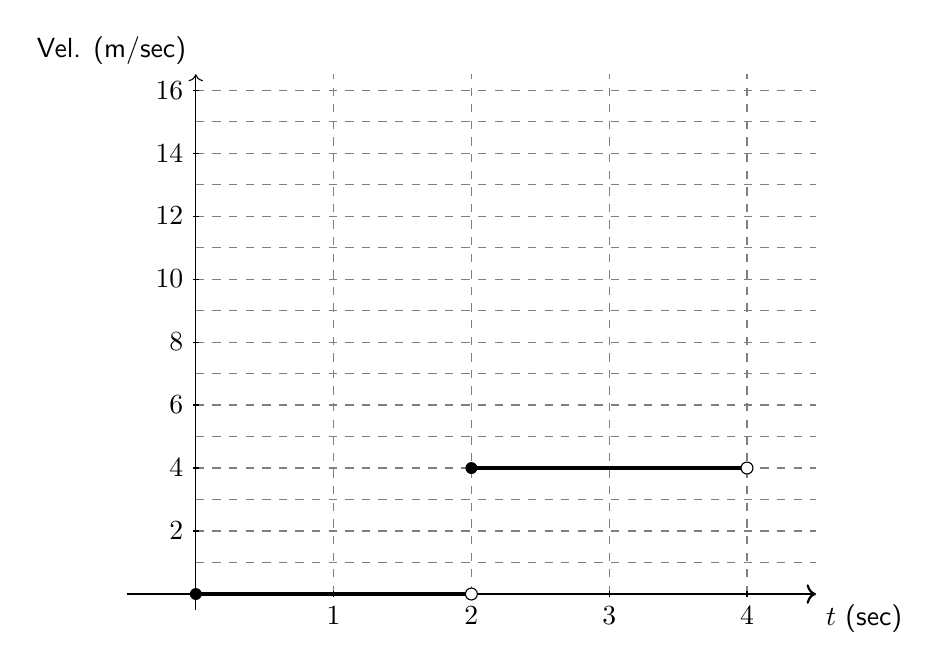
\begin{tikzpicture}[y=0.4cm, x=1.75cm,font=\sffamily]
    % ticks
    \draw[xstep = 1, ystep=1,gray,dashed] (0.0, 0.0) grid ( 4.5, 16.5);  %  very thin,opacity=0.85,
    % axis
    \draw[thick,->] (-0.5,0) -- coordinate (x axis mid) (4.5,0)  node[anchor = north west] {$t$ (sec)};
    \draw[->] (0,-0.5) -- coordinate (y axis mid) (0,16.5) node[anchor = south east] {Vel. (m/sec)};

      \foreach \y in {2,4,...,16} {
        \draw (1pt, \y) -- (-1pt, \y) node[anchor = east] {$\y$};
      }
      \foreach \x in {1,2,3,4} {
        \draw (\x,1pt) -- (\x,-1pt) node[anchor = north] {$\x$};
      }

     %\draw[scale=1.0,domain=0:5.1,smooth,variable=\x,very thick,black,samples=60]
    %    plot ({\x},{(\x)^2}); %node[anchor= west] {$f(x)=e^{ax}$};

    %\draw[pattern=crosshatch dots, pattern color=black,very thin,opacity=0.85] (1,0) rectangle (3,1);
    %\draw[pattern=crosshatch dots, pattern color=black,very thin,opacity=0.85] (3,0) rectangle (5,9);

     \draw[ultra thick] (0,0) -- (2,0);
     \fill[black] (0,0) circle [radius=0.5ex];
     \fill[white] (2,0) circle [radius=0.5ex];
     \draw (2,0) circle [radius=0.5ex];

     \draw[very thick] (2,4) -- (4,4);
     \fill[black] (2,4) circle [radius=0.5ex];
     \fill[white] (4,4) circle [radius=0.5ex];
     \draw (4,4) circle [radius=0.5ex];

    \end{tikzpicture}


  \begin{subproblem}
    \item Determine the total change in the position of the object
      from $t=0$ to $t=4$ seconds.
      \vfill
  \end{subproblem}
  \clearpage

\item A 2 kg object starts from rest on a straight track, and it can
  only move left or right. The positive direction is to the right, and
  the $\vec{i}$ component of the velocity is given in the plot below.

  %\scalebox{0.5}{\input{py/week8/piecewiseConstantVekII_week8day2.pgf}}

  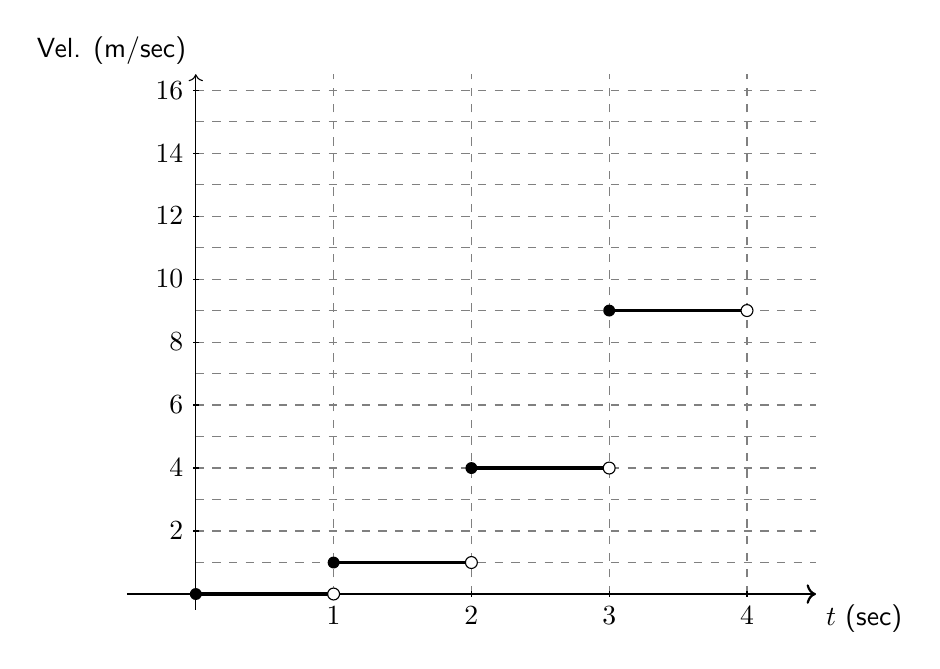
\begin{tikzpicture}[y=0.4cm, x=1.75cm,font=\sffamily]
    % ticks
    \draw[xstep = 1, ystep=1,gray,dashed] (0.0, 0.0) grid ( 4.5, 16.5);  %  very thin,opacity=0.85,
    % axis
    \draw[thick,->] (-0.5,0) -- coordinate (x axis mid) (4.5,0)  node[anchor = north west] {$t$ (sec)};
    \draw[->] (0,-0.5) -- coordinate (y axis mid) (0,16.5) node[anchor = south east] {Vel. (m/sec)};

      \foreach \y in {2,4,...,16} {
        \draw (1pt, \y) -- (-1pt, \y) node[anchor = east] {$\y$};
      }
      \foreach \x in {1,2,3,4} {
        \draw (\x,1pt) -- (\x,-1pt) node[anchor = north] {$\x$};
      }

     %\draw[scale=1.0,domain=0:5.1,smooth,variable=\x,very thick,black,samples=60]
    %    plot ({\x},{(\x)^2}); %node[anchor= west] {$f(x)=e^{ax}$};

    %\draw[pattern=crosshatch dots, pattern color=black,very thin,opacity=0.85] (1,0) rectangle (3,1);
    %\draw[pattern=crosshatch dots, pattern color=black,very thin,opacity=0.85] (3,0) rectangle (5,9);

     \draw[ultra thick] (0,0) -- (1,0);
     \fill[black] (0,0) circle [radius=0.5ex];
     \fill[white] (1,0) circle [radius=0.5ex];
     \draw (1,0) circle [radius=0.5ex];

     \draw[very thick] (1,1) -- (2,1);
     \fill[black] (1,1) circle [radius=0.5ex];
     \fill[white] (2,1) circle [radius=0.5ex];
     \draw (2,1) circle [radius=0.5ex];

     \draw[very thick] (2,4) -- (3,4);
     \fill[black] (2,4) circle [radius=0.5ex];
     \fill[white] (3,4) circle [radius=0.5ex];
     \draw (3,4) circle [radius=0.5ex];

     \draw[very thick] (3,9) -- (4,9);
     \fill[black] (3,9) circle [radius=0.5ex];
     \fill[white] (4,9) circle [radius=0.5ex];
     \draw (4,9) circle [radius=0.5ex];

    \end{tikzpicture}


  \begin{subproblem}
    \item Determine the total change in the position of the object
      from $t=0$ to $t=4$ seconds.
      \vfill
  \end{subproblem}

\end{problem}


\actTitle{Change in Position as Area}
\begin{problem}
\item A 2 kg object starts from rest on a straight track, and it can
  only move left or right. The positive direction is to the right, and
  the velocity at any time is $\vec{v}(t)=\vec{i} \; t^2$.

  \begin{subproblem}
    \item Make a sketch of the \textbf{velocity} in the $\vec{i}$
      direction using the axes below.

      %\scalebox{0.5}{\input{py/week8/changingVelGrid_week8day2.pgf}}
      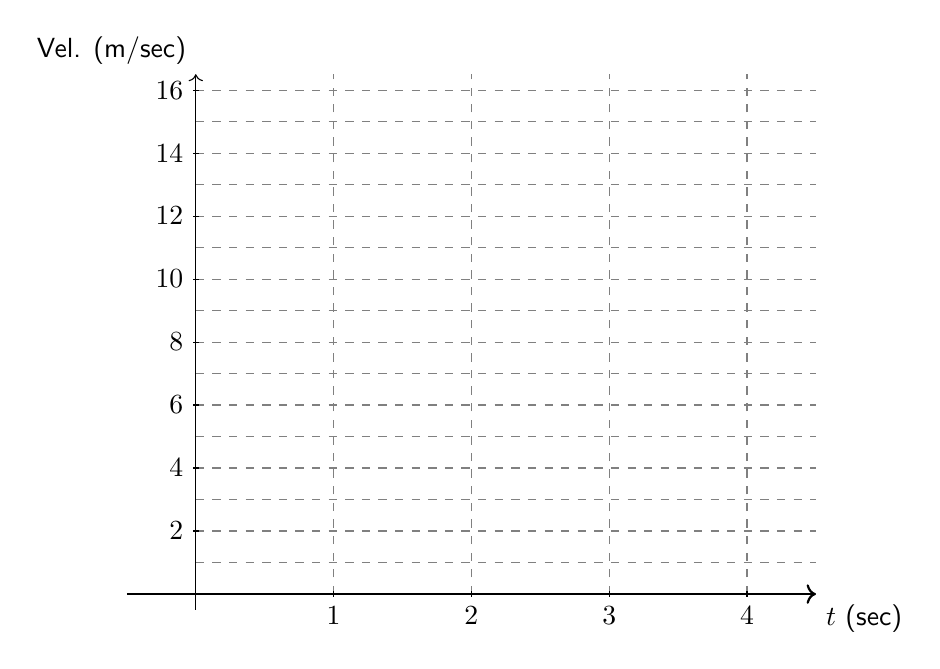
\begin{tikzpicture}[y=0.4cm, x=1.75cm,font=\sffamily]
        % ticks
        \draw[xstep = 1, ystep=1,gray,dashed] (0.0, 0.0) grid ( 4.5, 16.5);  %  very thin,opacity=0.85,
        % axis
        \draw[thick,->] (-0.5,0) -- coordinate (x axis mid) (4.5,0)  node[anchor = north west] {$t$ (sec)};
        \draw[->] (0,-0.5) -- coordinate (y axis mid) (0,16.5) node[anchor = south east] {Vel. (m/sec)};

          \foreach \y in {2,4,...,16} {
            \draw (1pt, \y) -- (-1pt, \y) node[anchor = east] {$\y$};
          }
          \foreach \x in {1,2,3,4} {
            \draw (\x,1pt) -- (\x,-1pt) node[anchor = north] {$\x$};
          }

         %\draw[scale=1.0,domain=0:5.1,smooth,variable=\x,very thick,black,samples=60]
        %    plot ({\x},{(\x)^2}); %node[anchor= west] {$f(x)=e^{ax}$};

        %\draw[pattern=crosshatch dots, pattern color=black,very thin,opacity=0.85] (1,0) rectangle (3,1);
        %\draw[pattern=crosshatch dots, pattern color=black,very thin,opacity=0.85] (3,0) rectangle (5,9);

        \end{tikzpicture}


    \item Determine the change in the position of the object after 4
      seconds by dividing up the time into four equally spaced
      intervals from $t=0$ to $t=4$ and assume that the force is constant over each
      interval. Sketch the assumed, piecewise constant velocity, on the
      axes above.
      \vfill
    \item Determine the change in position of the object after 4
      seconds by dividing up the time into eight equally spaced
      intervals from $t=0$ to $t=4$ and assume that the force is constant over each
      interval. Sketch the assumed, piecewise constant velocity, on the
      axes above.
      \vfill
  \end{subproblem}
  \clearpage

\item How can you improve the approximation in the previous activity?
  \vspace{3em}

\item Determine a way to express the approximation for the general
  case where there are $N$ intervals.

  \vfill

\end{problem}

\postClass

\begin{problem}
\item Briefly state two ideas from today's class.
  \begin{itemize}
  \item
  \item
  \end{itemize}
\item The position of an object is given by the equations
  below. Determine the velocity at any time.
  \begin{subproblem}
  \item $x(t) = e^{3t} + 4t  - 5$.
    \vfill
  \item $x(t) = 2\cos(\pi t) + \ln(t+2)$.
    \vfill
  \end{subproblem}
\item The velocity of objects are given by the equations
  below. Determine the position of each object. Assume each object
  starts at $x=1$m.
  \begin{subproblem}
  \item $v(t) = 3t - 5$.
    \vfill
  \item $v(t) = -2 t^3 + 10$.
    \vfill
  \end{subproblem}
\clearpage
\item The velocity of an object is
  \begin{eqnarray*}
    \vec{v}(t) & = & \cos(2t) \vec{i}.
  \end{eqnarray*}
  \begin{subproblem}
  \item Make a sketch of the velocity.
    \sideNote{ Be sure to label your axes and label all important
      points on your graph.}
    \vfill
  \item Express the change in the position from time 0 to time $T$ as
    a definite integral.
    \vfill
  \item Determine the change in the position from time 0 to time $T$
    by solving the definite integral.
    \vfill
  \item Make a sketch of the change in position and briefly describe
    the change in position.
    \sideNote{Be sure to label your axes and label all important
      points on your graph.}
    \vfill
  \end{subproblem}
  \clearpage

\item The velocity of an object is
  \begin{eqnarray*}
    \vec{v}(t) & = & \lp 5 - 5 e^{t/3} \rp \vec{i}.
  \end{eqnarray*}
  \begin{subproblem}
  \item Make a sketch of the velocity.  \sideNote{ Be sure to label
      your axes and label all important points on your graph.}
    \vfill
  \item Express the change in the position from time 0 to time $T$ as
    a definite integral.
    \vfill
  \item Determine the change in the position from time 0 to time $T$
    by solving the definite integral.
    \vfill
  \end{subproblem}
\end{problem}


%=========================================================================
% Start of activity on u substitution
%=========================================================================
\preClass{The Chain Rule}

\begin{problem}
\item Determine the derivatives of each the following functions. For
  the functions that have $u(t)$ keep the final answer in terms of
  $u'(t)$. In each case $C$ is a constant value.
  \begin{subproblem}
    \item $f(t) = e^{5t^2} + C$
      \vfill
    \item $f(t) = e^{u(t)} + C$
      \vfill
    \item $g(t) = t \cos(3t+6)  + C$
      \vfill
    \item $g(t) = t \cos(u(t))  + C$
      \vfill
    \item $h(t) = \ln\lp e^{8t} + 5 \rp  + C$
      \vfill
    \item $h(t) = \ln\lp u(t) \rp  + C$
      \vfill
  \end{subproblem}

\end{problem}


\actTitle{$u$-Substitution}
\begin{problem}
  \clearpage

\item The derivative of a function is given. Determine the
  anti-derivative of each function. In each case assume that $u=u(t)$
  is a function of $t$. \sideNote{Do not forget the constant!}
  \begin{subproblem}
  \item $F'(t) = \sin(u(t)) u'(t)$
    \vfill
  \item $G'(t) = e^{u(t)} u'(t)$
    \vfill
  \item $H'(t) = \frac{1}{u(t)} \cdot u'(t)$
    \vfill
  \end{subproblem}

  \clearpage

\item The force in Newtons acting on the car is given below. In each
  case determine the change in the momentum of the car from $t=0$ to
  $t=2$. \sideNote{Express the change as a definite integral and use
    the correct notation.}
  \begin{subproblem}
    \item $\vec{F} = \cos(\pi t) \vec{i}.$
      \vfill
    \item $\vec{F} = \lp 2 - 2 e^{t/9} \rp \vec{i}.$
      \vfill
    \item $\vec{F} = \frac{1}{t+1} \ln\lp t+1 \rp \vec{i}.$
      \vfill
  \end{subproblem}

\end{problem}

\postClass

\begin{problem}
\item Briefly state two ideas from today's class.
  \begin{itemize}
  \item
  \item
  \end{itemize}
\item Determine the derivatives of the following functions:
  %\sideNote{Leave the answer in terms of $u'(t)$.}
  \begin{subproblem}
  \item $f(t) = \cos(4t) + \ln(5t^2)$.
    \vfill
  \item $g(t) = \sin\lp e^{4t^5} \rp  + e^{\cos\lp 8t-5 \rp}$.
    \vfill
  \item $h(t) = \ln(4+\sin(2t) ) \cdot \cos \lp e^{2t^8} \rp$.
    \vfill
  \end{subproblem}

  \clearpage

\item A bag of sand lies on the floor, and its initial mass is 50
  kg. For each meter it is dragged sand is spilled, and it loses
  roughly 10\% of its mass each meter. The coefficient of friction
  between the bag and the floor is approximately $0.1$. A rope is
  attached to the bag, and the following force is applied to the bag
  \begin{eqnarray*}
    \vec{F}(t) & = & 10e^{-2t} \vec{i} + 20 e^{-2t} \vec{j}.
  \end{eqnarray*}
  How much work does the force exert on the bag?

  \vfill


\end{problem}

%=========================================================================
% Start of activities on practice of the ftc
%=========================================================================
\preClass{Definite Integrals}

\begin{problem}
\item For each function and bound determine the integral of the
  function geometrically as well as analytically. \sideNote{Make a
    sketch of the curve and indicate the signed area.}
  \begin{subproblem}
  \item $f(t)=t$ for $t=0$ to $t=1$.
    \vfill
  \item $g(t)=t+1$ for $t=0$ to $t=1$.
    \vfill
  \item $h(t)=-t$ for $t=0$ to $t=1$.
    \vfill
  %\item $f(t)=3t-4$ for $t=0$ to $t=2$.
  %  \vfill
  \end{subproblem}
\end{problem}


\actTitle{Impulse as a Definite Integral}
\begin{problem}
\item An object has a mass of 3 kg and rests on a flat table. It
  initially starts at rest at the point $\vec{x}=1\vec{i}$. It is
  subject to a force given by $\vec{F}(t) = \cos(\pi t) \vec{i}$.
  \begin{subproblem}
    \item Make a sketch of the free body diagram.
      \vspace{5em}
    \item Use the impulse/momentum theorem to determine the change in
      momentum of the object from $t=0$ to any time $t=T$.
      \vfill
    \item Solve the previous relationship for the velocity at any time
      and determine the position of the object at any time.
      \vfill
  \end{subproblem}

  \clearpage

\item A 3 kg object is initially located at $\vec{x}=1\vec{i}$ and
  starts from rest. Ignore the force due to friction between the
  object and the ground. A force of 10N is applied, and the angle
  changes uniformly from 0 radians to $\pi$ radians over a time of
  30 seconds.\\
  \includegraphics[width=7cm]{ink/week9/workAngleChanging}
  \begin{subproblem}
    \item Make a sketch of the free body diagram next to the diagram above.
    \item Determine the \textbf{work integral} that represents the
      work done by the force over the 30 second time span.  (Note that
      we are not yet able to determine the value of this integral.)
      \sideNote{Carefully move through the stages required to
        calculate a work integral. Carefully denote each step and
        briefly justify your choices.}

      \vfill

  \end{subproblem}
\end{problem}

\postClass

\begin{problem}
\item Briefly state two ideas from today's class.
  \begin{itemize}
  \item
  \item
  \end{itemize}
\item An object has a mass of 3 kg. It initially starts with a
  velocity of $2\vec{j}$ at the point $\vec{x}=1\vec{i}$. It is
  subject to a force given by $\vec{F}(t) = \sin(\pi t)\vec{j}$.
  \begin{subproblem}
    \item Make a sketch of the free body diagram.
      \vspace{5em}
    \item Use the impulse/momentum theorem to determine the change in
      momentum of the object from $t=0$ to any time $t=T$.
      \vfill
    \item Solve the previous relationship for the velocity at any time
      and determine the position of the object at any time.
      \vfill
  \end{subproblem}

  \clearpage

\item An object has a mass of 3 kg. It initially starts at rest with a
  velocity of $2\vec{j}$ at the point $\vec{x}=1\vec{i}$. It is
  subject to a force given by
  $\vec{F}(t) = \cos(\pi t)\vec{i}+\sin(\pi t)\vec{j}$.
  \begin{subproblem}
    \item Make a sketch of the free body diagram.
      \vspace{5em}
    \item Use the impulse/momentum theorem to determine the change in
      momentum of the object from $t=0$ to any time $t=T$.
      \vfill
    \item Solve the previous relationship for the velocity at any time
      and determine the position of the object at any time.
      \vfill
  \end{subproblem}
\end{problem}


%=========================================================================
% Start of activity on center of mass
%=========================================================================
\preClass{Areas Between Curves}

\begin{problem}
\item Determine the signed areas bounded by the curves described
  below. In each case first make a sketch of the region and then
  determine the integral. Determine the signed area geometrically
  rather than analytically if you are able to.
  \begin{subproblem}
  \item Above $y=1$, below $y=2x+1$, to the right of $x=0$ and to the
    left of $x=1$.
    \vfill
  \item Above $y=-1$, below $y=x+1$, to the right of $x=0$ and to the
    left of $x=2$.
    \vfill
  \end{subproblem}

\clearpage

\item An object has uniform density, and it is 0.1 m thick. Its mass
  is 1.2 kg. The object is bounded on the left by $x=0$, on the right by
  $x=6$, above by $y=7$, and below by $y=x$.
  \begin{subproblem}
    \item Make a sketch of the object.
      \vfill
    \item Determine the volume of the object geometrically.
      \vfill
    \item Determine the density of the object.
      \vfill
  \end{subproblem}


\end{problem}


\actTitle{Density and Center of Mass}
\begin{problem}

\item An object has uniform density, and it is 0.1 m thick. Its
  density is .5 kg/m\textsuperscript{3}. The object is bounded on the
  left by $x=0$, on the right by $x=6$, above by $y=7$, and below by
  $y=x$.
  \begin{subproblem}
    \item Make a sketch of the object. Show how you would subdivide
      the object for using an integral to determine the mass.
      \sideNote{Will you use vertical or horizontal strips?}
      \vfill
    \item Determine the mass of the object analytically.
      \sideNote{First derive the Riemann sum, take the limit, and then
        determine and solve the definite integral.}
      \vfill
    \item Determine the center of mass of the object.
      \vfill
  \end{subproblem}

  \clearpage

\item An object has uniform density, and it is 0.1 m thick. Its
  density is .6 kg/m\textsuperscript{3}. The object is bounded on the
  left by $x=0$, on the right by $x=1$, above by $y=x^2$, and below by
  $y=0$.
  \begin{subproblem}
    \item Make a sketch of the object. Show how you would subdivide
      the object for using an integral to determine the mass.
      \sideNote{Will you use vertical or horizontal strips?}
      \vfill
    \item Determine the mass of the object analytically.
      \sideNote{First derive the Riemann sum, take the limit, and then
        determine and solve the definite integral.}
      \vfill
    \item Determine the center of mass of the object.
      \vfill
  \end{subproblem}


\end{problem}

\postClass

\begin{problem}
\item Briefly state two ideas from today's class.
  \begin{itemize}
  \item
  \item
  \end{itemize}
\item An object has uniform density, and it is 0.1 m thick. Its mass
  is 10 kg. The object is bounded on the left by $x=0$, on the right
  by $x=5$, above by $y=x^2$, and below by $y=-x^2$.
  \begin{subproblem}
    \item Make a sketch of the object.
      \sideNote{Indicate how you are going to subdivide the object to
        calculate the volume.}
      \vfill
    \item Determine the volume of the object.
      \vfill
    \item Determine the density of the object.
      \vfill
  \end{subproblem}
  \clearpage

\item An object has a density that changes, and it is 0.1 m thick. Its
  density is uniform in the $z$ direction, and the density at a point
  $(x,y)$ is $\rho(x,y)=1+\sqrt{x}$ kg/m\textsuperscript{3}. The
  object is bounded on the left by $x=0$, on the right by $x=5$, above
  by $y=7$, and below by $y=x$.
  \begin{subproblem}
    \item Make a sketch of the object. Show how you would subdivide
      the object for using an integral to determine the mass.
      \sideNote{Will you use vertical or horizontal strips?}
      \vfill
    \item Determine the mass of the object analytically.
      \sideNote{First derive the Riemann sum, take the limit, and then
        determine and solve the definite integral.}
      \vfill
    \item Determine the center of mass of the object.
      \vfill
  \end{subproblem}
\end{problem}

%=========================================================================
% Start of day on optimization and kinematics
%=========================================================================
\preClass{Center of Mass}

\begin{problem}
\item An object has uniform density of 3 kg/m\textsuperscript{3}, and
  it is 0.1 m thick. The object has the shape of a rectangle that is
  2m tall and 0.1m wide. It is 0.1m thick.
  \begin{subproblem}
  \item Make a sketch of the object.
    \vfill
  \item Determine the volume of the object.
    \vfill
  \item Determine the mass of the object.
    \vfill
  \end{subproblem}
  \item An area is bounded on the left by $x=1$, on
  the right by $x=3$, above by $y=x$, and below by $y=-x$.
  Make a sketch of the object.
    \vfill
\end{problem}



\actTitle{Center of Mass With Varying Density}
\begin{problem}
\item A long, thin rod rests on the $x$-axis. The left end starts at
  $x=0$, and the other end goes to $x=4$ m. The density of the rod is
  $\rho(x)=1+\frac{x}{2}$ kg/m.
  \begin{subproblem}
  \item Make a sketch of the rod.
    \vspace{2em}
  \item Divide the rod into four parts, and approximate the total mass
    using a left sided Riemann sum.
    \vfill
  \item Divide the rod into $N$ parts and determine an expression for
    the left sided Riemann sum for the mass of the rod.
    \begin{subsubproblem}
      \item Determine the width of each piece in terms of $N$
        \vspace{3em}
      \item Determine the formula for the left endoint of each piece, $x_k$.
          \vfill
      \item Determine the mass of a single piece whose left endpoint is at $x_k$.
        \vfill
      \item Determine the Riemann sum that is an approximation of the total mass.
        \vfill
      \item Determine the definite integral that represents total mass.
          \sideNote{Do not determine the value of the integral just
            express the result as an integral.}
        \vspace{3em}
    \end{subsubproblem}

    \clearpage

  \item Repeat the previous steps to determine the total torque of the rod around
    the center of mass as an integral. First divide the rod into $N$ parts and determine an expression for
    the total torque of the pieces around the center of mass. (Denote
    the center of mass as $x_{\mathrm{cm}}$.)
    \vfill

  \item Set the previous expression to zero and solve  for the center of mass.
    \sideNote{Keep in mind that $x_{\mathrm{cm}}$ is a constant.}
    \vfill

  \end{subproblem}

  \clearpage

\item A metal plate is 0.1 m thick. The object is bounded on the left by
  $x=1$, on the right by $x=3$, above by $y=x$, and below by
  $y=-x$. The density of the object is $\rho(x)=1+\frac{x^2}{5}$
  kg/m. Determine the $x$-coordinate of the center of mass of the
  object.

  \vfill


\end{problem}

\postClass

\begin{problem}
\item Briefly state two ideas from today's class.
  \begin{itemize}
  \item
  \item
  \end{itemize}
\item A metal plate is 0.2 m thick. The object is bounded on the left by
  $x=2$, on the right by $x=5$, above by $y=x^2$, and below by
  $y=-x^2$. The density of the object is $\rho(x)=x+\frac{x^3}{10}$
  kg/m. Determine the $x$-coordinate of the center of mass of the
  object.
    \vfill
    \clearpage
\end{problem}


%=========================================================================
% Start of activity on work-energy as well as impulse relationships
%=========================================================================
\preClass{Work}

\begin{problem}
\item A rope is attached to an object, and it is pulled at an angle of
  $\frac{\pi}{6}$ from above the horizontal. The object is 3.0 kg, and
  the coefficient of friction is 0.3. The object is pulled for 3
  meters at a constant velocity. How much work was done by the force
  acting on the rope?

  \vfill
\end{problem}


\actTitle{Practice With Work Integrals}
\begin{problem}
\item A block is arranged as shown in the diagram below. The block has
  a mass of 50 kg, and its height, $H$, is 1m.  The coefficient of
  friction between the block and the base it is resting on is 0.2. A
  rope is connected to the block half way up and is hanging over a
  corner that has negligible friction. The right edge of the block is
  initially a distance $d_1=4.0$m from the edge, and it starts from
  rest. A constant tension of 150 N is applied to the rope. \\
  \includegraphics[width=7cm]{ink/week10/hangingBlocks}

  \begin{subproblem}
    \item Make a sketch of the free body diagram for the block.
      \vfill
    \item Determine the equations for Newton's Second Law in the $x$
      and $y$-directions.
      \vfill
      \clearpage
    \item Determine the equation for the acceleration in the
      horizontal direction.
      \vfill
    \item Use the fact that $\frac{d}{dt} x(t) = v(t)$ to write the
      equation in the previous question as a system of two equations
      in terms of $v(t)$ and $x(t)$.
      \vfill

      \clearpage

    \item Divide the \textbf{time} that the block is sliding into
      steps of 0.05 seconds. Approximate the position of the object at
      any time using a Riemann sum. (Use a spreadsheet to make the
      approximations.)

      \clearpage

  \end{subproblem}

  \clearpage

\item Using the previous situation determine an approximation of the
  work done by the force of friction on the upper block from the start
  and until it reaches the corner.

  \vfill

\end{problem}

\postClass

\begin{problem}
\item Briefly state two ideas from today's class.
  \begin{itemize}
  \item
  \item
  \end{itemize}
\item
  \begin{subproblem}
    \item
  \end{subproblem}
\end{problem}

%=========================================================================
% Start of session on trig review
%=========================================================================
\preClass{Trig Review}

\begin{problem}
\item Determine the derivatives of each of the following functions:
  \begin{subproblem}
  \item $\sin(3t)$
    \vfill
  \item $\cos(3t)$
    \vfill
  \item $\tan(3t)$
    \vfill
  \item $\sin(t)\cos(t)$
    \vfill
  \end{subproblem}

  \clearpage

\item Determine the lengths and angles of the parts of the triangles
  that are missing in each of the triangles below.

  \scalebox{0.5}{%% Creator: Matplotlib, PGF backend
%%
%% To include the figure in your LaTeX document, write
%%   \input{<filename>.pgf}
%%
%% Make sure the required packages are loaded in your preamble
%%   \usepackage{pgf}
%%
%% Figures using additional raster images can only be included by \input if
%% they are in the same directory as the main LaTeX file. For loading figures
%% from other directories you can use the `import` package
%%   \usepackage{import}
%% and then include the figures with
%%   \import{<path to file>}{<filename>.pgf}
%%
%% Matplotlib used the following preamble
%%   \usepackage{fontspec}
%%   \setmainfont{Bitstream Vera Serif}
%%   \setsansfont{Bitstream Vera Sans}
%%   \setmonofont{Bitstream Vera Sans Mono}
%%
\begingroup%
\makeatletter%
\begin{pgfpicture}%
\pgfpathrectangle{\pgfpointorigin}{\pgfqpoint{8.000000in}{6.000000in}}%
\pgfusepath{use as bounding box, clip}%
\begin{pgfscope}%
\pgfsetbuttcap%
\pgfsetmiterjoin%
\definecolor{currentfill}{rgb}{1.000000,1.000000,1.000000}%
\pgfsetfillcolor{currentfill}%
\pgfsetlinewidth{0.000000pt}%
\definecolor{currentstroke}{rgb}{1.000000,1.000000,1.000000}%
\pgfsetstrokecolor{currentstroke}%
\pgfsetdash{}{0pt}%
\pgfpathmoveto{\pgfqpoint{0.000000in}{0.000000in}}%
\pgfpathlineto{\pgfqpoint{8.000000in}{0.000000in}}%
\pgfpathlineto{\pgfqpoint{8.000000in}{6.000000in}}%
\pgfpathlineto{\pgfqpoint{0.000000in}{6.000000in}}%
\pgfpathclose%
\pgfusepath{fill}%
\end{pgfscope}%
\begin{pgfscope}%
\pgfpathrectangle{\pgfqpoint{1.000000in}{0.600000in}}{\pgfqpoint{6.200000in}{4.800000in}} %
\pgfusepath{clip}%
\pgfsetbuttcap%
\pgfsetmiterjoin%
\pgfsetlinewidth{1.003750pt}%
\definecolor{currentstroke}{rgb}{0.000000,0.000000,0.000000}%
\pgfsetstrokecolor{currentstroke}%
\pgfsetdash{}{0pt}%
\pgfpathmoveto{\pgfqpoint{1.281818in}{3.000000in}}%
\pgfpathlineto{\pgfqpoint{4.100000in}{3.000000in}}%
\pgfpathlineto{\pgfqpoint{4.100000in}{4.745455in}}%
\pgfpathlineto{\pgfqpoint{1.281818in}{3.000000in}}%
\pgfusepath{stroke}%
\end{pgfscope}%
\begin{pgfscope}%
\pgfpathrectangle{\pgfqpoint{1.000000in}{0.600000in}}{\pgfqpoint{6.200000in}{4.800000in}} %
\pgfusepath{clip}%
\pgfsetbuttcap%
\pgfsetmiterjoin%
\pgfsetlinewidth{1.003750pt}%
\definecolor{currentstroke}{rgb}{0.000000,0.000000,0.000000}%
\pgfsetstrokecolor{currentstroke}%
\pgfsetdash{}{0pt}%
\pgfpathmoveto{\pgfqpoint{4.381818in}{3.000000in}}%
\pgfpathlineto{\pgfqpoint{6.918182in}{3.000000in}}%
\pgfpathlineto{\pgfqpoint{6.918182in}{5.181818in}}%
\pgfpathlineto{\pgfqpoint{4.381818in}{3.000000in}}%
\pgfusepath{stroke}%
\end{pgfscope}%
\begin{pgfscope}%
\pgfpathrectangle{\pgfqpoint{1.000000in}{0.600000in}}{\pgfqpoint{6.200000in}{4.800000in}} %
\pgfusepath{clip}%
\pgfsetbuttcap%
\pgfsetmiterjoin%
\pgfsetlinewidth{1.003750pt}%
\definecolor{currentstroke}{rgb}{0.000000,0.000000,0.000000}%
\pgfsetstrokecolor{currentstroke}%
\pgfsetdash{}{0pt}%
\pgfpathmoveto{\pgfqpoint{1.281818in}{0.818182in}}%
\pgfpathlineto{\pgfqpoint{4.100000in}{0.818182in}}%
\pgfpathlineto{\pgfqpoint{4.100000in}{2.781818in}}%
\pgfpathlineto{\pgfqpoint{1.281818in}{0.818182in}}%
\pgfusepath{stroke}%
\end{pgfscope}%
\begin{pgfscope}%
\pgfpathrectangle{\pgfqpoint{1.000000in}{0.600000in}}{\pgfqpoint{6.200000in}{4.800000in}} %
\pgfusepath{clip}%
\pgfsetbuttcap%
\pgfsetmiterjoin%
\pgfsetlinewidth{1.003750pt}%
\definecolor{currentstroke}{rgb}{0.000000,0.000000,0.000000}%
\pgfsetstrokecolor{currentstroke}%
\pgfsetdash{}{0pt}%
\pgfpathmoveto{\pgfqpoint{4.381818in}{0.818182in}}%
\pgfpathlineto{\pgfqpoint{6.918182in}{0.818182in}}%
\pgfpathlineto{\pgfqpoint{6.918182in}{2.345455in}}%
\pgfpathlineto{\pgfqpoint{4.381818in}{0.818182in}}%
\pgfusepath{stroke}%
\end{pgfscope}%
\begin{pgfscope}%
\pgfpathrectangle{\pgfqpoint{1.000000in}{0.600000in}}{\pgfqpoint{6.200000in}{4.800000in}} %
\pgfusepath{clip}%
\pgfsetrectcap%
\pgfsetroundjoin%
\pgfsetlinewidth{1.003750pt}%
\definecolor{currentstroke}{rgb}{0.000000,0.000000,0.000000}%
\pgfsetstrokecolor{currentstroke}%
\pgfsetdash{}{0pt}%
\pgfpathmoveto{\pgfqpoint{3.818182in}{3.000000in}}%
\pgfpathlineto{\pgfqpoint{3.818182in}{3.218182in}}%
\pgfpathlineto{\pgfqpoint{4.100000in}{3.218182in}}%
\pgfusepath{stroke}%
\end{pgfscope}%
\begin{pgfscope}%
\pgfpathrectangle{\pgfqpoint{1.000000in}{0.600000in}}{\pgfqpoint{6.200000in}{4.800000in}} %
\pgfusepath{clip}%
\pgfsetrectcap%
\pgfsetroundjoin%
\pgfsetlinewidth{1.003750pt}%
\definecolor{currentstroke}{rgb}{0.000000,0.000000,0.000000}%
\pgfsetstrokecolor{currentstroke}%
\pgfsetdash{}{0pt}%
\pgfpathmoveto{\pgfqpoint{6.636364in}{3.000000in}}%
\pgfpathlineto{\pgfqpoint{6.636364in}{3.218182in}}%
\pgfpathlineto{\pgfqpoint{6.918182in}{3.218182in}}%
\pgfusepath{stroke}%
\end{pgfscope}%
\begin{pgfscope}%
\pgfpathrectangle{\pgfqpoint{1.000000in}{0.600000in}}{\pgfqpoint{6.200000in}{4.800000in}} %
\pgfusepath{clip}%
\pgfsetrectcap%
\pgfsetroundjoin%
\pgfsetlinewidth{1.003750pt}%
\definecolor{currentstroke}{rgb}{0.000000,0.000000,0.000000}%
\pgfsetstrokecolor{currentstroke}%
\pgfsetdash{}{0pt}%
\pgfpathmoveto{\pgfqpoint{3.818182in}{0.818182in}}%
\pgfpathlineto{\pgfqpoint{3.818182in}{1.036364in}}%
\pgfpathlineto{\pgfqpoint{4.100000in}{1.036364in}}%
\pgfusepath{stroke}%
\end{pgfscope}%
\begin{pgfscope}%
\pgfpathrectangle{\pgfqpoint{1.000000in}{0.600000in}}{\pgfqpoint{6.200000in}{4.800000in}} %
\pgfusepath{clip}%
\pgfsetrectcap%
\pgfsetroundjoin%
\pgfsetlinewidth{1.003750pt}%
\definecolor{currentstroke}{rgb}{0.000000,0.000000,0.000000}%
\pgfsetstrokecolor{currentstroke}%
\pgfsetdash{}{0pt}%
\pgfpathmoveto{\pgfqpoint{6.636364in}{0.818182in}}%
\pgfpathlineto{\pgfqpoint{6.636364in}{1.036364in}}%
\pgfpathlineto{\pgfqpoint{6.918182in}{1.036364in}}%
\pgfusepath{stroke}%
\end{pgfscope}%
\begin{pgfscope}%
\pgftext[x=1.620000in,y=3.043636in,left,base]{\sffamily\fontsize{14.000000}{16.800000}\selectfont \(\displaystyle \pi/3\)}%
\end{pgfscope}%
\begin{pgfscope}%
\pgftext[x=3.818182in,y=4.178182in,left,base]{\sffamily\fontsize{14.000000}{16.800000}\selectfont \(\displaystyle 0.6\)}%
\end{pgfscope}%
\begin{pgfscope}%
\pgftext[x=1.338182in,y=4.527273in,left,base]{\sffamily\fontsize{20.000000}{24.000000}\selectfont A}%
\end{pgfscope}%
\begin{pgfscope}%
\pgftext[x=4.720000in,y=3.043636in,left,base]{\sffamily\fontsize{14.000000}{16.800000}\selectfont \(\displaystyle \pi/6\)}%
\end{pgfscope}%
\begin{pgfscope}%
\pgftext[x=6.551818in,y=4.178182in,left,base]{\sffamily\fontsize{14.000000}{16.800000}\selectfont \(\displaystyle 0.5\)}%
\end{pgfscope}%
\begin{pgfscope}%
\pgftext[x=4.269091in,y=4.527273in,left,base]{\sffamily\fontsize{20.000000}{24.000000}\selectfont B}%
\end{pgfscope}%
\begin{pgfscope}%
\pgftext[x=1.620000in,y=0.861818in,left,base]{\sffamily\fontsize{14.000000}{16.800000}\selectfont \(\displaystyle \theta\)}%
\end{pgfscope}%
\begin{pgfscope}%
\pgftext[x=3.592727in,y=1.123636in,left,base]{\sffamily\fontsize{14.000000}{16.800000}\selectfont \(\displaystyle 0.5\)}%
\end{pgfscope}%
\begin{pgfscope}%
\pgftext[x=2.550000in,y=1.909091in,left,base]{\sffamily\fontsize{14.000000}{16.800000}\selectfont \(\displaystyle 0.4\)}%
\end{pgfscope}%
\begin{pgfscope}%
\pgftext[x=1.338182in,y=2.345455in,left,base]{\sffamily\fontsize{20.000000}{24.000000}\selectfont C}%
\end{pgfscope}%
\begin{pgfscope}%
\pgftext[x=4.720000in,y=0.861818in,left,base]{\sffamily\fontsize{14.000000}{16.800000}\selectfont \(\displaystyle \theta\)}%
\end{pgfscope}%
\begin{pgfscope}%
\pgftext[x=5.565455in,y=0.861818in,left,base]{\sffamily\fontsize{14.000000}{16.800000}\selectfont \(\displaystyle 0.5\)}%
\end{pgfscope}%
\begin{pgfscope}%
\pgftext[x=5.368182in,y=1.690909in,left,base]{\sffamily\fontsize{14.000000}{16.800000}\selectfont \(\displaystyle 0.4\)}%
\end{pgfscope}%
\begin{pgfscope}%
\pgftext[x=4.269091in,y=2.345455in,left,base]{\sffamily\fontsize{20.000000}{24.000000}\selectfont D}%
\end{pgfscope}%
\end{pgfpicture}%
\makeatother%
\endgroup%
}

  \vfill

\end{problem}

\actTitle{Derivatives of Other Trigonometric Functions}
\begin{problem}

\item We examine the identity
  \begin{eqnarray*}
    \sin^2(\theta) + \cos^2(\theta) & = & 1.
  \end{eqnarray*}

  \begin{subproblem}
  \item Make a sketch of the unit circle. Use the definition of sine
    and cosine to explain why the identity above is true.
    \sideNote{Just give a heuristic explanation.}
    \vfill

  \item Divide both sides of the identity by $\cos^2(\theta)$.
    \vfill

  \item Use the definition of the tangent and secant to express the
    new result in terms of these two trigonometric functions.
    \vfill

  \end{subproblem}

  \clearpage

\item We derive the derivative of $\sec(\theta)$.

  \begin{subproblem}
    \item Express $\sec(\theta)$ in terms of the cosine.
      \vspace{4em}
    \item Determine the derivative of the previous expression.
      \vfill
    \item Use any appropriate trigonometric identity to simplify the
      expression.
      \vfill
  \end{subproblem}
  \clearpage

\item We derive the derivative of $\cot(\theta)$.

  \begin{subproblem}
    \item Express $\cot(\theta)$ in terms of the sine and the cosine.
      \vspace{4em}
    \item Determine the derivative of the previous expression.
      \vfill
    \item Use any appropriate trigonometric identity to simplify the
      expression.
      \vfill
  \end{subproblem}
  \clearpage

\end{problem}

\postClass

\begin{problem}
\item Briefly state two ideas from today's class.
  \begin{itemize}
  \item
  \item
  \end{itemize}
\item A person is standing at the origin, $(0,0)$, and they are facing
  in the positive $x$-direction. The person turns to the left
  $\frac{\pi}{3}$ radians, walks 3 meters in 10 seconds. The person
  stops, turns $\frac{\pi}{4}$ to the right and walks 5 meters in
  another 10 seconds.
  \begin{subproblem}
    \item  Make a sketch of the person's path.
      \vfill
    \item Determine the person's position at 10 and 20 seconds.
      \vfill
    \item Determine the person's position for any time less than 10
      seconds.
      \vfill
    \item Determine the person's position for any time between 10 and
      20 seconds.
      \vfill
  \end{subproblem}
  \clearpage
\item A person is standing at the origin, $(0,0)$, and they are facing
  in the positive $x$-direction. The person turns to the left
  $\frac{2\pi}{3}$ radians, walks 3 meters in 10 seconds. The person
  stops, turns $\frac{\pi}{2}$ to the left and walks 5 meters in
  another 10 seconds.
  \begin{subproblem}
    \item  Make a sketch of the person's path.
      \vfill
    \item Determine the person's position at 10 and 20 seconds.
      \vfill
    \item Determine the person's position for any time.
      \vfill
  \end{subproblem}
\end{problem}


%%% Local Variables:
%%% mode: latex
%%% TeX-master: "labManual"
%%% End:


%\chapter{Circular Motion}
%%=========================================================================
% Start of activity on simple harmonic motion.
%=========================================================================
\preClass{Derivatives of Basic Trigonometric Functions}

\begin{problem}
\item Determine the derivatives of the following functions:
  \begin{subproblem}
  \item $\sin(3t)$
    \vfill
  \item $\cos(8t)$
    \vfill
  \end{subproblem}
\item Determine the anti-derivatives of the following functions:
  \begin{subproblem}
  \item $\cos(3t)$
    \vfill
  \item $\sin(8t)$
    \vfill
  \end{subproblem}

\clearpage

\item An object has an acceleration given by
  \begin{eqnarray*}
    a(t) & = & 2\sin(5t) + 5e^{-2t},
  \end{eqnarray*}
  and the initial velocity is $v_0$, and the initial position is $x_0$.
  \begin{subproblem}
  \item Determine the position at any time.
    \vfill
  \item Describe the qualitative behaviour of the position. Does the position
    oscillate, grow, or decay? For what values of $v_0$ and $x_0$ do
    you see different behaviours?
    \vfill
  \end{subproblem}

\end{problem}


\actTitle{Simple Harmonic Motion}
\begin{problem}

\item An object is attached to a rigid spring on a frictionless
  horizontal table. The origin is determined to be the equilibrium
  position for the object. The mass of the object is 3kg. The object
  is drawn back 0.05m and released from rest. The spring obeys Hooke's
  law with a constant, $k=0.4$N/m.
  \begin{subproblem}
    \item Make a sketch of the physical situation.
      \vfill
    \item Make a sketch of the free body diagram. Ignore any friction
      assuming that the friction is negligible for now.
      \vfill
    \item Describe the qualitative behaviour that you expect to see
      from the physical system. How should it behave?
      \vfill
    \item Determine the equation of motion in the $x$-direction
      ignoring friction.  
      \vfill

    \item Based on your description of the expected behaviour what
      kind of function mimics that behaviour?
      \vspace{3em}

      \clearpage

    \item Assume that the solution has the form
      \begin{eqnarray*}
        x(t) & = & A \sin(\omega t) + B \cos(\omega t),
      \end{eqnarray*}
      where $A$, $B$, and $\omega$ are constants. 
      \sideNote{It is not uncommon to just make a guess at a general
        form, and then check to see if your intuition is consistent
        with the equation.}
      \begin{subproblem}
      \item Determine the velocity and acceleration based on the
        position above.  
        \vfill
      \item Substitute these results into your equation for the motion
        of the object.
        \vfill
        \clearpage
      \item Put all of the sines on one side of the equality and all
        of the cosines on the other side of the equality. What must be
        true about the left and right hand sides?
        \sideNote{Hint: It has to be true for \textbf{all} time!}
        \vspace{6em}
      \item Is it possible to determine values for the constants to
        satisfy the equation and the initial conditions? If so what
        are they?
        \sideNote{Hint: Yes.}
        \vfill
      \end{subproblem}

  \end{subproblem}
\end{problem}

\postClass

\begin{problem}
\item Briefly state two ideas from today's class.
  \begin{itemize}
  \item 
  \item 
  \end{itemize}
\item Determine the first and second derivatives of the following functions.
  \begin{subproblem}
  \item $8\sin(5t)$
    \vfill
  \item $23\cos(2t)$
    \vfill
  \item $8\sin(5t)+2\cos(5t)$
    \vfill
  \item $23\cos(2t)-14\sin(2t)$
    \vfill
  \end{subproblem}
\end{problem}

%=========================================================================
% Start of activity on finding optimal values of a parameter in SHM
%=========================================================================
\preClass{Simple Harmonic Motion}

\begin{problem}
\item Determine the solution to the following differential equations.
  \begin{subproblem}
  \item $x'' + 4 x  =  0$, $x(0)=0$, $v(0)=1$.
    \vfill
  \item $x'' + 8 x  =  0$, $x(0)=1$, $v(0)=0$.
    \vfill
  \end{subproblem}
\end{problem}


\actTitle{Optimization For Simple Harmonic Motion - Determining The System}
\begin{problem}
\item A spring mass system is to be constructed. The system will be
  assembled on a horizontal table, and friction is ignored. 
  \begin{subproblem}
    \item Make a sketch of the physical situation.
      \vfill
    \item Make a sketch of the free body diagram. Ignore any friction
      assuming that the friction is negligible for now. Assume that
      the spring constant is $k$ N/m and the mass is $m$ kg.
      \vfill
    \item Describe the qualitative behaviour that you expect to see
      from the physical system. How should it behave?
      \vfill
    \item Determine the equation of motion ignoring friction.
      \vfill
  \end{subproblem}

  \clearpage

\item We now have the general equations of motion for a spring-mass
  system with parameters $k$ and $m$. The goal is to determine values
  of $k$ and $m$ so that the first time \textbf{after} it is in motion
  the system reaches its maximum distance away from the origin in 0.1
  seconds. Assume that the object is first pulled 0.3 m from
  equilibrium and released from rest. What is the constraint for $k$
  and $m$?

  \vfill

\item The cost of the spring depends on $k$ and is $(1+2k)$\$. The cost of
  the object depends on its mass and is $10(m+k^2)$\$. What is the
  total cost of building the system?

  \vspace{4em}

\item Formally express the cost and objective functions:
    \begin{eqnarray*}
      \mathrm{Minimize:} & &  \\
      \mathrm{Constraint:} & & 
    \end{eqnarray*}



\end{problem}


\postClass

\begin{problem}
\item Briefly state two ideas from today's class.
  \begin{itemize}
  \item 
  \item 
  \end{itemize}


\item Rewrite the system from this set of activities.
    \begin{eqnarray*}
      \mathrm{Minimize:} & &  \\
      \mathrm{Constraint:} & & 
    \end{eqnarray*}
    \begin{subproblem}
    \item Make a sketch of the constraint.  \sideNote{ Be sure to
        label your axes and label all important points on your graph.}

      \vfill

    \item Add a sketch of the cost functions for various values of the
      cost. What is the general pattern? Make a prediction for the
      optimal values of $k$ and $m$.

      \vspace{3em}
    \end{subproblem}
\clearpage

\item Rewrite the system from this set of activities.
  \begin{eqnarray*}
    \mathrm{Minimize:} & &  \\
    \mathrm{Constraint:} & & 
  \end{eqnarray*}

  \begin{subproblem}
  \item Analytically determine the optimal values of $k$ and $m$.
    \vfill
  \end{subproblem}
\end{problem}

%=========================================================================
% Start of activities on systems of equations
%=========================================================================
\preClass{Linearizations}

\begin{problem} 
\item We examine the linearization of the function
  \begin{eqnarray*}
    f(x) & = & x^2-4.
  \end{eqnarray*}
  \begin{subproblem}
  \item Draw a set of axes where $-2\leq x \leq 2$. 

    \sideNote{ Be sure to label your axes and label all important
      points on your graph.}

    \vfill

  \item Make a sketch of the function $f(x)$ on the axes.
  \item Add a sketch of the tangent line to the function at $x=1$.
  \item Determine the formula for the tangent line at $x=1$.
    \vfill

  \end{subproblem}
\end{problem}


\actTitle{Approximating Solutions to Nonlinear Equations}
\begin{problem}
\item We will examine a way to determine an estimate for the value of
  $x$ that satisfies $0=x^2-4$.
  \begin{subproblem}
  \item Draw a set of axes where $-2\leq x \leq 2$. 

    \sideNote{ Be sure to label your axes and label all important
      points on your graph.}

    \vfill

  \item Make a sketch of the relationship $f(x)=x^2-4$ on the axes.
  \item Suppose you cannot determine the value of $x$ where $f(x)=0$,
    and you make an initial estimate that $x=1$ is a root. Add a
    sketch of the tangent line to the function at $x=1$.

  \item Mark the point where the height of the \textbf{tangent line}
    is zero. Is this new $x$ value a better or worse approximation for the value of
    $x$?  

    \vspace{2em}

    \clearpage


  \item Determine analytically the tangent line to the graph of the
    curve at the initial estimate for the root, $x=1$. Determine the
    value of $x$ where the height of the tangent line is zero.

    \vfill


  \item Add sketch of another tangent line at the new value of $x$ to
    your original plot on the previous page. 

  \item Mark the point where the height of the \textbf{tangent line}
    is zero. Is this new $x$ value a better or worse approximation for the value of
    $x$?  

    \vspace{2em}

  \item Determine analytically the tangent line to the graph of the
    curve at the new estimate for the root. Determine the value of $x$
    where the height of this new tangent line is zero.

    \vfill


  \item Add sketch of another tangent line at the new value of $x$ to
    your original plot on the previous page. 

  \item Mark the point where the height of the \textbf{new tangent line}
    is zero. Is this new $x$ value a better or worse approximation for
    the value of $x$?


  \end{subproblem}

  \clearpage

\item Determine an algorithm to calculate the tangent line to a
  function at $x=a$, and find the value of $x$ where the tangent line
  is zero.

  \vfill

\clearpage

\item Use your algorithm multiple times to find an approximation to
  the square root of 4 with an initial estimate of $x=1$.

  \vfill

\item How do you know when to stop applying the algorithm and your
  approximation is ``close?''

\end{problem}


\postClass

\begin{problem}
\item Briefly state two ideas from today's class.
  \begin{itemize}
  \item 
  \item 
  \end{itemize}
\item We will graphically determine the values of $x$ and $y$ that
  satisfy both of the following equations:
  \begin{eqnarray*}
    x^2 + y  & = & 0, \\
    x - 2y^2 & = & 1.
  \end{eqnarray*}

  \begin{subproblem}
  \item Draw a set of axes where $-3\leq x \leq 3$ and $-3 \leq y \leq
    3$. 

    \sideNote{ Be sure to label your axes and label all important
      points on your graph.}

    \vfill

  \item Make a sketch of the relationship $x^2+y=0$ on the axes.
  \item Make a sketch of the relationship $x-2y^2=1$ on the axes.
  \item Circle and estimate the points where both relationships are
    satisfied.
  \end{subproblem}
\clearpage
\item Determine the values of $x$ and $y$ that satisfy both of the
  following equations:
  \begin{eqnarray*}
    x + 4y & = & 7, \\
    x + 3y & = & 5.
  \end{eqnarray*}
  \clearpage
\item We will graphically determine the values of $x$ and $y$ that
  satisfy both of the following equations:
  \begin{eqnarray*}
    x + 4y & = & 7, \\
    x + 3y & = & 5.
  \end{eqnarray*}
  \begin{subproblem}
  \item Draw a set of axes where $-3\leq x \leq 3$ and $-3 \leq y \leq
    3$. 

    \sideNote{ Be sure to label your axes and label all important
      points on your graph.}

    \vfill

  \item Make a sketch of the relationship $x+4y=7$ on the axes.
  \item Make a sketch of the relationship $x+3y=5$ on the axes.
  \item Circle and estimate the points where both relationships are
    satisfied.
  \end{subproblem}
\end{problem}

%=========================================================================
% Start of activity on riemann sums and moment of intertia
%=========================================================================
\preClass{Moment of Inertia}

\begin{problem}
\item A point mass of 2 kg is located at $3\vec{i} + 2\vec{j}$, and a
  point mass of 4 kg is located at $-\vec{i}+3\vec{j}$. Determine the
  moment of inertia around the $x$-axis as well as the moment of
  inertia around the $y$-axis  of the system.

  \vfill

  \clearpage


\item A set of ten point masses is lined up on the $x$ axis. They are
  positioned at $x_n=n\cdot 0.1$ where $n=0,~1,\ldots,9$. The mass of
  each point mass is $\frac{n}{2}$ kg.
  \begin{subproblem}
    \item Make a rough sketch of the system.
      \vfill
    \item Determine the center of mass of the system.
      \vfill
    \item Determine the moment of inertia of the system around the
      $y$-axis.
      \vfill
  \end{subproblem}


\end{problem}


\actTitle{Moment of Inertia for Continuous Masses}
\begin{problem}
\item A thin metal rod is located on the $x$-axis. The left side of
  the rod is located at $x=0$m and the right hand side is located at
  $x=1$m. The density of the rod is given by $\rho(x)=5x$ kg/m.
  \begin{subproblem}
    \item Make a rough sketch of the system.
      \vfill
    \item Divide it up into $n$ equal sized small segments. Determine
      the location of the left hand side of each small segment.
      \vfill
    \item Determine an approximation for the density of each small
      segment.
      \vfill
    \item Determine the approximate mass and the moment of inertia for
      each small segment.  
      \vfill

      \clearpage

    \item Determine the sum that can be used to approximate the center
      of mass and the sum that can be used to approximate the moment
      of inertia.

      \vspace{5em}

    \item Determine the center of mass and the moment of inertia for
      the rod.

      \vfill

  \end{subproblem}
\end{problem}

\postClass

\begin{problem}
\item Briefly state two ideas from today's class.
  \begin{itemize}
  \item 
  \item 
  \end{itemize}
\item Relate the sum for the center of mass with the integral. Make a
  plot and discuss the relationship with the sum with the area under a
  function. (Which function are you finding the area under?)

  \vfill
\end{problem}


%=========================================================================
% Start of day on moment of inertia and angular momentum.
%=========================================================================
\preClass{Constant Angular Velocity}

\begin{problem}
\item An object moves around a circle with a constant angular
  velocity, $\omega$, and a constant distance from the origin,
  $r$. The initial angle, $\theta$, is zero.
  \begin{subproblem}
  \item Determine the angle at any time.
    \vfill
  \item Determine the position at any time.
    \sideNote{Use proper vector notation.}
    \vfill
  \item Determine the derivative of the position at any time.
    \vfill
  \item What is the magnitude of the velocity vector?
    \vfill
  \end{subproblem}

  \clearpage

\item An object moves around a circle of radius $r$  at a constant
  rate, $\theta=\omega t$. Its position at any time is $\vec{r}$.

  \begin{subproblem}
    \sideNote{Draw the vector $\delta\vec{r}$ in the plot.}
  \item based on the plot below to graphically represent the
    difference in the positions between any times, $\vec{r}(t+\delta
    t)-\vec{r}(t)$. Blow up, redraw, and focus just on the two
    positions on the circle.

    \includegraphics[width=7cm]{ink/week12/circularAcceleration}

    \vfill

    \sideNote{Draw the velocity vectors and then sketch the difference.}
  \item Graphically represent the difference in the velocity vectors,
    $\vec{v}(t+\delta t)-\vec{v}(t)$, at the two positions in the plot
    below. Blow up, redraw, and focus just on the two positions on the
    circle.

    \includegraphics[width=7cm]{ink/week12/circularAcceleration}

    \vfill

  \end{subproblem}

\end{problem}


\actTitle{Energy Associated With Constant Angular Velocity}
\begin{problem}
\item An object moves around a circle of radius $r$  at a constant
  rate, $\theta=\omega t$. Its position at any time is $\vec{r}$.

  \begin{subproblem}
  \item Determine the position at any time. Express the position as
    a vector.
    \sideNote{Assume that $\omega$ is constant.} \\
    \includegraphics[width=7cm]{ink/week12/circularMotion}
    \vfill
  \item Determine the velocity and the acceleration by taking the
    derivatives of the position with respect to time.
    \vfill
  \item Using the velocity vector determine the energy of the object
    at any time.
    \vfill
  \end{subproblem}

  \clearpage

\item An object whose position is given by $\vec{r}(t)$ is moving in
  two dimensions. The angle between the velocity and the position is
  $\theta$ as shown in the diagram below. The velocity can be
  expressed by two components, one in the direction of the position
  vector and the other direction
  perpindicular to the position vector. \\
  \includegraphics[width=7cm]{ink/week12/angularComponents}
  \begin{subproblem}
  \item Determine the magnitude of
    the component of the velocity that is parallel to the position
    vector and the magnitude of the component of the velocity that is
    perpendicular to the position vector.  \vfill
  \item Determine the magnitude of the vector given by
    $\vec{r}\times\vec{v}$.
    \vfill
  \item The magnitude of the component $\vec{v}$ that is perpindicular
    to $\vec{r}$ is equal to the magnitude of $\vec{r}$ multiplied by
    the magnitude of the angular velocity, $\vec{\omega}$.  Use the
    previous expressions to determine the magnitude of $\vec{\omega}$
    in terms of $\vec{r}\times\vec{v}$ and $\vec{r}$.  
    \vfill
  \end{subproblem}
  \clearpage
\item An object moves around a circle of radius $r$  at a constant
  rate, $\theta=\omega t$. Its position at any time is $\vec{r}$.
  \begin{subproblem}
  \item Rewrite the vectors for the position and velocity from the
    previous activity.
    \vfill
  \item Determine the value of $\vec{r}\times\vec{v}$.
    \vfill
  \item Determine the value of $\vec{r}\times\vec{v}$ divided by the
    square of the magnitude of $\vec{r}$.
    \vfill
  \item Which direction is the result?
    \vfill
  \end{subproblem}
\end{problem}

\postClass

\begin{problem}
\item Briefly state two ideas from today's class.
  \begin{itemize}
  \item 
  \item 
  \end{itemize}
\item for each image below make a rough sketch of the missing
  component, $\vec{r}$, $\vec{v}$, or $\vec{\omega}$.
  \begin{subproblem}
  \item \includegraphics[width=7cm]{blender/week12/negativeZOmega}
  \item \includegraphics[width=7cm]{blender/week12/findOmega}
  \item \includegraphics[width=7cm]{blender/week12/positiveZOmega}
  \end{subproblem}
\end{problem}


%=========================================================================
% Start of activity on angular velocity for simple and non-simple
% harmonic motion.
%=========================================================================
\preClass{Constant Angular Velocity}

\begin{problem}
%\item A mass is moving in a circle of radius $R$ at a constant speed,
%  $v$.
%  \begin{subproblem}
%  \item Draw a picture of the path and include the free body diagram.
%    \vfill
%  \item Add the acceleration of the object in your plot above. In
%    which direction is the acceleration?
%    \vfill
%  \item What is the magnitude of the acceleration?
%    \vfill
%  \item How will the diagram change if the velocity is not constant?
%    \vfill
%  \end{subproblem}
%
%\clearpage

\item The position of a mass is
  $\vec{r}(t)=r\cos(\omega t)\vec{i}+r\sin(\omega t)\vec{j}$. The
  value of $\omega$ is a constant.
  \begin{subproblem}
  \item Draw a sketch of the object's path. Include the start point
    and the direction of travel of the object.
    \vfill
  \item How long does it take to complete one full revolution?
    \vspace{3em}
  \item Determine the velocity and acceleration. Add a sketch of the
    vectors to your plot above.
    \vfill
    \clearpage
  \item Determine the value of $|\vec{a}(t)|$ using your results for
    the velocity and acceleration above.  
    \vfill
  \item Determine the value of $\frac{|\vec{v}(t)|^2}{|\vec{r}(t)|}$
    using your results for the velocity and acceleration above.
    \vfill
  \end{subproblem}

\end{problem}

\actTitle{Non-constant Angular Velocity}
\begin{problem}
\item The position of a mass is
  $\vec{r}(t)=r\cos(\omega t^2)\vec{i}+r\sin(\omega t^2)\vec{j}$. The
  value of $\omega$ is a constant.
  \begin{subproblem}
  \item Draw a sketch of the object's path. Include the start point
    and the direction of travel of the object.
    \vfill
  \item Determine the velocity and acceleration. Add a sketch of the
    vectors to your plot above.
    \vfill
    \clearpage
  \item Is the relationship $\frac{|\vec{v}(t)|^2}{|\vec{r}(t)|}$
    still valid?
    \vfill
  \item Determine the radial component, $\vec{a}_r(t)$, of the
    acceleration.
    \vfill
  \item Show that $|\vec{a}_r(t)| = \frac{|\vec{v}(t)|^2}{|\vec{r}(t)|}$
    \vfill
  \end{subproblem}
\end{problem}

\postClass

\begin{problem}
\item Briefly state two ideas from today's class.
  \begin{itemize}
  \item 
  \item 
  \end{itemize}
\item The position of a mass is
  $\vec{r}(t)=r\cos(\omega t)\vec{i}+r\sin(\omega t)\vec{j}$. The
  value of $\omega$ is a constant.
  \begin{subproblem}
  \item Draw a sketch of the object's path. Include the start point
    and the direction of travel of the object.  
    \vfill
    \vfill
  \item Find the distance that the mass travels from time $t=0$ to a
    later time, $t=T$.
    \vfill
  \item What happens as the value of $\omega$ changes? For example
    if you double $\omega$ what happens to the distance? What does
    that imply about the speed?
    \vfill
  \end{subproblem}
\end{problem}


%=========================================================================
% Start of day on the derivative of inverse functions
%=========================================================================
\preClass{Inverse Trigonometric Functions}

\begin{problem}
\item Make a sketch of the unit circle. Mark and label the points on
  the circle that correspond to the angles $\frac{\pi}{4}$,
  $\frac{\pi}{3}$, and $\frac{3\pi}{4}$.
  \vfill
  \vfill
\item If the sine of an angle is $\frac{\sqrt{2}}{2}$ what are all
  possible values of the angle?
  \vfill
\item If the sine of an angle is $\frac{\sqrt{3}}{2}$ what are all
  possible values of the angle?
  \vfill
\end{problem}


\actTitle{The Derivative of the Inverse of a Function}
\begin{problem}
\item Suppose that
  \begin{eqnarray}
    \label{eqn:arcsin}
    y &= & \arcsin(t),
  \end{eqnarray}
  assuming that $t$ is between $\frac{-\pi}{2}$ and $\frac{\pi}{2}$.
  \begin{subproblem}
  \item Solve equation \ref{eqn:arcsin} for $t$ as a function of
    $y$.
    \vfill
  \item Assuming that $y$ is a function of $t$ use the chain rule to
    determine the derivative of $y(t)$ with respect to $t$.  
    \vfill
  \item Use the identity $\sin^2(y)+\cos^2(y)=1$ to express $y'(t)$ in
    terms of $\sin(y)$.  
    \vfill
  \item Use the definition of $y(t)$ to determine $y'(t)$ only in
    terms of $t$.  
    \vfill

  \end{subproblem}

  \clearpage

\item Suppose that
  \begin{eqnarray}
    \label{eqn:inverseFunction}
    y &= & f^{-1}(t).
  \end{eqnarray}
  \begin{subproblem}
  \item Solve equation \ref{eqn:inverseFunction} for $t$ as a function
    of $y$.
    \vfill

  \item Assuming that $y$ is a function of $t$ use the chain rule to
    determine the derivative of $y(t)$.  
    \vfill

  \item Solve the previous expression for $y'(t)$.
    \vfill

  \end{subproblem}


\end{problem}

\postClass

\begin{problem}
\item Briefly state two ideas from today's class.
  \begin{itemize}
  \item 
  \item 
  \end{itemize}

\item Use the result on the derivative of the inverse to show that the
  derivative of the square root function satisfies
  \begin{eqnarray*}
    \frac{d}{dt} \sqrt{t} & = & \frac{1}{2\sqrt{t}}.
  \end{eqnarray*}

  \vfill

\item Use the result on the derivative of the inverse to determine the
  derivative of the inverse cosine function.
  \vfill

\item Use the result on the derivative of the inverse to show that the
  derivative of the natural logarithm satisfies
  \begin{eqnarray*}
    \frac{d}{dt} \ln(t) & = & \frac{1}{t}.
  \end{eqnarray*}

  \vfill


\end{problem}




%%% Local Variables:
%%% mode: latex
%%% TeX-master: "labManual"
%%% End:


\chapter{GNU Free Documentation License}
\include{fdl-1.3}

\end{document}
